\documentclass[11pt]{article}
\usepackage{times}
\usepackage{verbatim}
\usepackage[pdftex]{graphicx}    
\usepackage[pdftex]{color}  
\usepackage{fullpage}
\usepackage{url}

\usepackage[numbers,sort&compress]{natbib}

% \draftfalse: submission version. Legends,tables at end. No figs included.
% \drafttrue:   online preprint. Figures and table inline.
\newif\ifdraft
%\draftfalse
\drafttrue

\renewcommand{\baselinestretch}{1.5}
\setcounter{secnumdepth}{0}

\begin{document}

\title{Filter sensitivity targeting for RNA similarity searches}
\author{Eric P. Nawrocki and Sean R. Eddy\\
HHMI Janelia Farm Research Campus\\
19700 Helix Drive\\
Ashburn VA 20147\\
\url{http://selab.janelia.org/}\\
}
%\date{\today}
\maketitle

%abstract
\section{Motivation:}
Covariance models (CMs) are profile probabilistic models for RNA
similarity search that score both sequence and secondary structure
conservation.  The practical application of CMs has been limited by
the high computational complexity of their dynamic programming search
algorithms.

\section{Results:}
We present a filtering technique for CM searches called filter
sensitivity targeting (FST) that determines filter thresholds to
maximize speed while maintaining a target level of sensitivity. When
applied to HMM filtering, FST speeds up CM searches by about 25-fold
while sacrificing very little sensitivity on our benchmark.

\section{Availability:}
Source code and documentation downloadable from
\href{http://infernal.janelia.org}. Freely licensed under the GNU
General Public License version 3 (GPLv3).

\textbf{Contact:} \url{{nawrockie,eddys}@janelia.hhmi.org}

\section{Introduction}

\software{infernal} is a software package that allows you to make
consensus RNA secondary structure profiles, and use them to search
nucleic acid sequence databases for homologous RNAs, or to create new
structure-based multiple sequence alignments.

To make a profile, you need to have a multiple sequence alignment of
an RNA sequence family, and the alignment must be annotated with a
consensus RNA secondary structure. The program \prog{cmbuild} takes an
annotated multiple alignment as input, and outputs a profile.

You can then use that profile to search a sequence database for homologs,
using the program \prog{cmsearch}.

You can also use the profile to align a set of unaligned sequences to
the profile, producing a structural alignment, using the program
\prog{cmalign}. This allows you to build hand-curated representative
alignments of RNA sequence families, then use a profile to
automatically align any number of sequences to that profile.  This
seed alignment/full alignment strategy combines the strength of
stable, carefully human-curated alignments with the power of automated
updating of complete alignments as sequence databases grow. This is
the strategy used to maintain the \database{Rfam} database of RNA
multiple alignments and profiles.

\software{infernal} is comparable to \software{hmmer}
(\htmladdnormallink{hmmer.janelia.org}{http://hmmer.janelia.org}).  The
\software{hmmer} software package builds profile hidden Markov models
(profile HMMs) of multiple sequence alignments. Profile HMMs capture
only primary sequence consensus features. \software{infernal} models
are profile stochastic context-free grammars (profile SCFGs).  Profile
SCFGs include both sequence and RNA secondary structure consensus
information.

Currently \software{infernal} is really just an algorithm
testbed. Output is rudimentary, and some desired features are
missing. Most importantly, \software{infernal} is very slow and
CPU-intensive. You will probably need a large number of CPUs in order
to use it for serious work. Planned algorithmic improvements should
make it more practical in the future. We are making it available as a
fully documented package now, only because \software{infernal} has
been pressed prematurely into service as the basis for constructing
and maintaining the \database{Rfam} database of structurally annotated
RNA multiple alignments \cite{Griffiths-Jones03}. When we assign a 1.0
release number, that's when we'll think \software{infernal} is ready
for prime time. Until then, please bear with us.













\section{Approach}

We propose a technique for determining filter survival thresholds that
will achieve any target level of sensitivity. This technique, which we
call filter sensitivity targeting (FST), is similar to
Weinberg/Ruzzo's rigorous filters and Zhang/Bafna's keyword filters in
that it prioritizes sensitivity over speed, but differs in that it
does not provably sacrifice zero sensitivity. A potential advantage
of FST over the other methods is that it may be faster (by pruning away
more of the database) while sacrificing an acceptably small amount of
sensitivity.  
% SOMETHING HERE ABOUT HOW FILTER THRESHOLDS ARE FINAL THRESHOLD DEPENDENT?
First, we describe the general FST procedure, which can be applied to
any type of filter for any type of similarity search method. Then we
focus on the application of FST to HMM filtering for RNA similarity
searches with CMs.

%---------------------------------------------------------------------
\begin{comment}
We propose a new filtering strategy that prioritizes sensitivity over
speed, but does not provably sacrifice zero sensitivity like
Weinberg/Ruzzo rigorous filters or Zhang/Bafna keyword filters.
Instead, our method, which we call filter sensitivity targeting (FST),
determines filter thresholds that will theoretically achieve a
pre-defined target level of sensitivity with the filter. FST is a
general procedure that can be applied to any type of filter for any
type of similarity search method, but here we focus on HMM filtering
for CM searches for structural RNAs.
\end{comment}
%---------------------------------------------------------------------

%%%%%%%%%%%%%%%%%%%%%%%%%%%%%%%%%%%%%%%%%%%%%%%%%%%%%%%%%%%%%%%%%%%%%%

\subsection{Determining filter survival thresholds by filter sensitivity
  targeting (FST)} 

Filtered database searches involve two search algorithms, which we
will refer to as the \emph{filter} algorithm and the \emph{final}
algorithm. The database is scored first with the filter algorithm,
and surviving subsequences, or hits, are rescored with the final algorithm.
%---------------------------------------------------------------------
\begin{comment}
%A filtered database search involves two algorithms:
%the full database is first searched using the \emph{filter} algorithm
%and surviving sequences are then searched with the \emph{final} search algorithm.
Filtered database searches involve (at least) two search algorithms,
which we will refer to as the \emph{filter} algorithm and the
\emph{final} algorithm. The database is searched first with the filter
algorithm, and surviving subsequences are searched with the final
algorithm.
%The following terms are relevant to our discussion of FST:

\begin{description}
\item[$C$: final reporting score threshold] the minimum score of a
  database subsequence that will be reported by the final search
  algorithm as a plausible hit.
\item[$T$: filter survival score threshold] the minimum score required
  of a database subsequence to survive the filter, and subsequently be
  searched with the final search algorithm.
\item[$F$: filter sensitivity] the fraction of database subsequences that
  score above $C$ using the final search method and also score above
  $T$ using the filter.
\end{comment}
%---------------------------------------------------------------------
We define the sensitivity $F$ of a filter as the fraction of database
hits that survive the filter (score above a filter survival score
threshold $T$) that a non-filtered search with only the final algorithm
would report (score above a reporting score threshold $C$).  FST is a
procedure for estimating the appropriate 
%filter survival threshold 
$T$ to use to achieve $F$ sensitivity for a search using threshold
$C$. The only required input of the procedure is the desired $F$, and
a set of $N$ test sequences. There are three main steps to FST:

\begin{enumerate}
\item
  Score $N$ test sequences using both the filter and final algorithms.
\item
  Create two lists of the sequences. Sort list 1 by increasing final
  score. Sort list 2 by increasing filter score.
\item
  For sequence $i=1$ to $N$, with final score $C_i$, in list 1:
\begin{itemize}
\item
  Prune list 2 to only include the $(N-i+1)$ sequences with final score
  $>=C_i$
\item
  Set the filter threshold $T_i$ equal to the $(F*(N-i+1))$
  ranked filter score from pruned list 2. 
\item
  Save $(T_i,C_i)$ as a filter survival threshold/final reporting
  threshold score pair.
\end{itemize}
\end{enumerate}

When finished, each $(T,C)$ pair indicates a filter survival score
threshold $T$ to use when searching with final reporting threshold $C$
to theoreatically achieve filter sensitivity $F$.  If the test
sequences are a representative sample of the real target homologous
sequences, then in the limit of very large $N$ and infinite database
searching, using $(T,C)$ in this way will achieve sensitivity $F$.
In other words, the larger and more representative of real homologs
the set of test sequences is, the more accurate, and consequently
useful, the FST approach is. 

A caveat to the procedure is that in step 3, as $i$ approaches $N$, ($N-i$), 
the number of test sequences used to determine $T_i$, approaches
zero. Because the accuracy of FST depends on the number of test
sequences being large, it's reasonable to set a max on $i$, in
practice we use $0.9 * N$, so that at least $0.1*N$ test sequences are
used to determine all $(T,C)$ pairs.

Figure~\ref{Fig:fst} shows data for the FST procedure for three
anecdotal RNA families using $N=10,000$ and $F=0.993$. Each small
point represents a sequence, with x-coordinate equal to filter score
and y-coordinate equal to final score. The larger points are a subset
of the $(T,C)$ pairs. For each $(T,C)$ point, the fraction of
small points with $y>C$ that have $x<T$ is $1-F=0.007$, these represent
the $0.7\%$ of sequences that a non-filtered search would find that a
filtered search will not find. 

\subsection{Source of test sequences}
%This leads to the question of how to obtain the test sequences. 
An important question is: how do we obtain the test sequences?  One
approach is to use known examples of homologs.  Weinberg and Ruzzo
essentially suggested a special case of the FST strategy to define
thresholds for ML HMM filters for CM searches by using the
\textsc{Rfam} ``seed'' sequences as the $N$ sequences and requiring an
$F$ of $1.0$. (They ultimately decided on using filter survival
thresholds that would eliminate $99\%$ of the target database as their
thresholding strategy.) The seed sequences are the sequences in the
\textsc{Rfam} structural alignment used to build the
CM. Alternatively, the \textsc{Rfam} ``full'' sequences could be used,
which are all the sequences that score above an expertly curated score
threshold (chosen as the score of the highest scoring obvious false
positive) in a BLAST filtered CM search of the RFAMSEQ database.

For structural RNAs, there are two drawbacks to using known homologs
as the $N$ test sequences.  First, the number of known homologs is
usually small. The median number of seed plus full sequences per RNA
family in \textsc{Rfam} release 9.1 (by far the largest public
database of RNAs) is 50, with 100 or more sequences in 30\% of the
families, and 1000 or more sequences in only 6\%.  This is problematic
because the accuracy of FST depends on $N$ being large.  Secondly,
known homologs are unlikely to be a representative sample of the
sequences the CM would classify as homologous with stastically
significant scores.  Alignments of the seed sequences are used to
build and paramterize the models themselves, and as a result those
sequences are a biased sample of very high scoring sequences.  The
full sequences have been detected using a BLAST filter and,
presumably, are also a biased, high scoring sample (although it is
impossible to be certain without doing a prohibitively expensive
non-filtered CM search for comparison).  CM parameterization has
recently been significantly improved for remote homology detection
\citep{NawrockiEddy07}, with the adaptation of informative mixture
Dirichlet priors and entropy weighting from profile HMM
implementations. In order for a FST calibrated filter to maintain that
increased sensitivity, the test sequences must include lower scoring,
but still statistically significant, remotely homologous sequences.

An alternative source of the test sequences is to take advantage of
the generative capacity of CMs as probabilistic models and sample the
test sequences directly from the model.  This approach addresses the
requirements of our strategy. $N$ can be large because sampling is
fast and infinitely repeatable, and sampling draws sequences from the
CM's own probability distribution, which is exactly the distribution
of homologs the CM is modelling.  Figure~\ref{Fig:hists} illustrates
the difference in the CM score distributions of random sequences
(solid lines), known (\textsc{Rfam} seed \emph{and} full sequences,
dotted lines), and sampled sequences (dashed lines) for three
anecdotal RNA families: tRNA, 5S rRNA, and SRP RNA. In all three
cases, the known sequences are biased towards high scores relative to
the sampled sequences.

%Note that for all three families the range of scores that are
%significantly better than random is more widely covered by the
%score distribution of sampled sequences than by the score distribution
%of known sequences. 

\subsection{Scoring and sampling sequences}

CM similarity search algorithms assign a bit score to a target
database subsequence. The bit score $B$ is a log odds score: $B =
\log_2 \frac {P( \mbox{seq} | \mbox{CM})} { P (\mbox{seq} |
  \mbox{null})}.$ $P( \mbox{seq} | \mbox{CM})$ is the probability of a
target subsequence according to the CM. The \emph{Inside} dynamic
programming algorithm calculates this value by summing the probability
of all possible paths $\pi$ through the model that generate the
subsequence, that is: $P( \mbox{seq} | \mbox{CM} ) = \sum_{\pi} P(
\mbox{seq}, \pi | \mbox{CM}).$ \citep{Durbin98}.  $P (\mbox{seq} |
\mbox{null}) $ is the probability of the target sequence given a
``null hypothesis'' model of the statistics of random sequence. The
null model is a simple one-state hidden Markov model (HMM) that says
that random sequences are i.i.d. sequences with a specific residue
composition, which is equiprobable across the four RNA nucleotides
($0.25$ each).  Therefore the null model score is calculated as: $ P
(\mbox{seq} | \mbox{null}) = 0.25^L$ for a sequence of length
$L$. Because this null model score depends only on the length of the
target sequence, and not the sequence itself, $B$ increases
monotonically with $P( \mbox{seq}, \pi | \mbox{CM})$ for a constant
$L$.  As the probability that a sequence was generated from the CM
increases, so does it's score. This suggests that sampling from the
disbribution defined by: $P ( \mbox{seq}, \pi | \mbox{CM} )$ should
yield high scoring sequences.  This is confirmed anecdotally for three
families in Figure~\ref{Fig:hists} for which the scores of the vast
majority of sampled sequences are significantly better than random.

Sampling a sequence from a CM is a recursive procedure that begins at
the root state and samples a tree of states, called a parsetree, and
sequence residues, until all branches of the tree terminate at end
states. The emitted sequence associated with a parsetree is generated
from outside to inside (as opposed to from left to right from an
HMM). When singlet or basepair emitting states are visited a single
residue or basepair residue, respectively, is sampled from the state's
emission probability distribution. If the emitting state is a singlet
left-emitting state, the sampled residue is appended on the right (3')
to the left half of the nascent sequence. Conversely, if the emitting
state is a singlet right-emitting state, the sampled residue is
appended on the left (5') to the right half of the sequence. Basepair
states behave as both a left-emitting and right-emitting state,
emitting one residue to the left and one to the right. Finally, when
bifurcation states are visited, two new paths are created, one
beginning at the left child state and one at the right child state,
and each of these paths is continued until an end state is reached.
The time complexity of the sampling procedure is $O(N)$ time for a CM
of $N$ states. Roughly 10,000 paths can be sampled from average sized
CM per second.

CMs can be locally or globally configured
\citep{KleinEddy03,infguide03}. In global mode, the only way to enter
and exit the model is through the root state and end states,
respectively.  In local mode, begins and ends are possible from any
internal node of the model. Further, when a local end takes place, a
special insert state is visited that can emit additional
sequence. Local ends allow CMs to tolerate insertions or deletions of
entire substructures, increasing sensitivity for remote homology
detection in some cases.

\subsection{Practical limits on filter survival thresholds}

When finding survival threshold $T$, %to achieve a target sensitivity,
FST prioritizes sensitivity over speed by ignoring the
effect using $T$ will have on the running time of a filtered search. 
%The FST procedure prioritizes sensitivity over speed by empirical
%determination of an appropriate $T$ to achieve a target sensitivity
%while ignoring the effect that $T$ will have on the running time of
%the filtered search. 
We can further prioritize sensitivity over speed by enforcing a
maximally useful filter survival threshold $T_{max}$, and to use
$min(T, T_{max})$ for any FST derived $T$. This can only increase the
sensitivity of the filter (because $T_{max} < T$) at a cost to
speed. However, $T_{max}$ can be chosen so that the effect on the total
running time is negligible.%, as described next.

The running time ($t$) of a filtered search is the time required to
run the filter on the full target ($t_f$) plus the time required to
run the final algorithm on the full target ($t_m$) multiplied by the
fraction that survives the filter ($S$).  That is, $t = t_f + S *
t_m$.  The survival fraction $S$ is controlled by the survival
threshold $T$: as $T$ increases, $S$ decreases, and vice versa.  
%The relationship between $T$ and $S$ is query dependent. 
Because $t$ is directly affected by $S$, a reasonable way to enforce a
$T_{max}$ is to use a single query independent $S_{min}$, and
converting it to a $T_{max}$ for each query. This requires a way of
converting between $S$ and $T$, which is straightforward if E-values
are available: $S=\frac{EL}{Z}$, where $E$ is the E-value for $T$
using the filter scoring algorithm, $Z$ is the database size, and $L$
is the average length of a surviving fraction of the database from the
filter. The appropriate choice of $S_{min}$ is likely to be highly
dependent on the ratio of running times of the filter and final scoring
algorithms. We investigate reasonable $S_{min}$ values to use for HMM
filtered CM searches based on empirical performance in a benchmark
below.

\subsection{Using the banded CYK algorithm as a second filter}
In some cases, using two filters in succession, or \emph{chain}
filtering, can compound the resulting acceleration without sacrificing
sensitivity \citep{Zhang06}.
%This is especially true if the two filtering techniques differ
%significantly in speed and efficiency.
Previously, we developed a banded version of the CYK dynamic
programming (DP) algorithm for CM similarity search called
query-dependent banding (QDB) \citep{NawrockiEddy07} that
precalculates regions of the DP lattice that have negligible
probability and ignores those regions during the DP recursion for
greater speed. In our benchmarks, QDB offered about a four-fold
speedup at a small cost to sensitivity. This work on filtering led us
to reevaluate the primary use of QDB CYK, testing it as a filter for
the more sensitive and time consuming Inside algorithm, instead of as
a standalone, final algorithm for similarity search.  Rather than use
FST to determine thresholds for CYK filtering, we tried a simpler,
query-independent strategy of setting the filter E-value threshold as
100 times the final algorithm threshold. We discuss our results below.

%%%%%%%%%%%%%%%%%%%%%%%%%%%%%%%%%%%%%%%%%%%%%%%%%%%%%%%%%%%%%%%%%%
% UNUSED (CURRENTLY)

\begin{comment}
CM dynamic programming search algorithms (CYK and Inside) scale $O(L N^3)$ for
query RNA length $N$ and database length $L$. HMM algorithms scale
$O(L N)$; $O(N^2)$ slower than CM algorithms. 
The vast majority (1370 of 1372) of RNA families in Rfam
(release 9.1) have $N < 1000$. Even for models of length $1000$,
assuming equally efficient implementations of CM and HMM algorithms,
a CM search would theoretically take $10^6$ times as long as an
HMM. In this case $t_m/t_f = 10^6$.

defining a $T_{max}$ value equates to defining a $S_{min}$ value. 

The
minimum possible time required for a filtered search is $t_f$, which
equals $t$ when $S=0$. The difference in running time between two
filtered searches using $S_1$ and $S_2$ is $|(S_1-S_2)| *
t_m$. Because the minimum possible running time $t_f$ is achieved when
$S=0$, the maximum cost in time for using $S_{min}$ instead of $S <
S_{min}$ is $S_{min}*t_m$. If $S_{min}*t_m$ is a ``negligible'' cost
relative to the minimally possible time $t_f$, then enforcing
$S_{min}$, and the corresponding $T_{max}$ value, will have a
negligible effect on the running time. For example, if
$S_{min} = 0.01 * t_f/t_m$, then enforcing $S_{min}$ and it's
corresponding $T_{max}$ will yield a running time only 1\% slower
than a filter-only search.


$S*t_m$ is significantly smaller than $t_f$, using $S' < S$ will
result in an insignificantly faster running time. 

$t_1 = t_f + S_1 * t_m$
$t_2 = t_f + S_2 * t_m$
$t_1 - t_2 = (t_f + S_1 * t_m) - (t_f + S_2 * t_m)$
$t_1 - t_2 = S_1 * t_m - S_2 * t_m$
$t_1 - t_2 = (S_1 - S_2) * t_m$
$T_min < T$, using it as a threshold can only increase the sensitivity
of the filter,  

 by setting
$T_min$ that will result in an $S$ is sufficiently small, such that 
$(t_f + S * t_m) - t_f <$
 lower $S$ would have 


The survival fraction $S$ for a given $T$ is query-dependent

 as a
function of the filter running time, $t_{min} = X * t_f$ (with $X$
necessarily greater than $1$.
For example, setting $X=2$, means that the target filtered search time
is twice the time a filter-only search would take, anything faster is
unnecessary.  
A $t_{min}$ value implies an $S_{min}$ value: $t_{min} = t_f + S_{min} * t_m$,
and it follows that $S_{min} = \frac{X-t_f}{t_m}$.
%This gives us a way to set a minimum $S$ for a filtered search to
%achieve a minimum running time of $X*t_f$ based on the 

To combine this technique with FST thresholds requires a way to convert
between a survival threshold $T$ to a survival fraction $S$. One way
to do this is to use \emph{E-value} statistics, which will convert $T$
to an expected number of hits expected by random at or above $T$. The
only other required values are $L$, the expected length of a surviving
chunk of database that includes a hit, and $Z$ the size of the
database. This gives $E_{min} = \frac{S_{min}*Z}{L}$. Finally
$E_{min}$ can be converted to $T_{max}$ using E-value
statistics. $T_{max}$ is the maximally useful survival score
threshold; the predicted running time of a search with $T_{max}$ is $X * t_f$. 
To apply the technique, when using an FST derived $T$ for a filtered
search, replace it with $T_max$ if $T > T_{max}$.
\end{comment}

%-------------------------------------------------------------
\begin{comment}
Another way to prioritize sensitivity over speed
is to set a minimally useful, target running time $t_{min}$ as a
function of the filter running time, $t_{min} = X * t_f$, with $X>1$.
For example, setting $X=2$, means that the target filtered search time
is twice the time a filter-only search would take, anything faster is
unnecessary.  
A $t_{min}$ value implies an $S_{min}$ value: $t_{min} = t_f + S_{min} * t_m$,
and it follows that $S_{min} = \frac{X-t_f}{t_m}$.
%This gives us a way to set a minimum $S$ for a filtered search to
%achieve a minimum running time of $X*t_f$ based on the 

To combine this technique to FST thresholds requires a way to convert
between a survival threshold $T$ to a survival fraction $S$. One way
to do this is to use \emph{E-value} statistics, which will convert $T$
to an expected number of hits expected by random at or above $T$. The
only other required values are $L$, the expected length of a surviving
chunk of database that includes a hit, and $Z$ the size of the
database. This gives $E_{min} = \frac{S_{min}*Z}{L}$. Finally
$E_{min}$ can be converted to $T_{max}$ using E-value
statistics. $T_{max}$ is the maximally useful survival score
threshold; the predicted running time of a search with $T_{max}$ is $X * t_f$. 
To apply the technique, when using an FST derived $T$ for a filtered
search, replace it with $T_max$ if $T > T_{max}$.
\end{comment}
%-------------------------------------------------------------
\begin{comment}
The goal of FST is to determine thresholds $T$ that will achieve a target
sensitivity while minimizing the running time of the search.  However
by setting a minimum time for the search, 

For example, if the target search time is $2t_f$ (the filtered search
takes twice as long as a filter only search), then $S_{min}=t_f/t_m$. 
More generally, if a target search time is set as $X * t_f$ (with $X >
1$, then $S_{min} = \frac{X-t_f}{t_m}$. 

Enforcing $S_{min}$ for a filtered search effectively ignores the FST
calibrated threshold $T$ by using a $T_max < T$. But this is only done
when it comes a negligible (predicted) cost in running time, and
because $T_max < T$, filter sensitivity can only increase.

Let $t_{f}$ and $t_{c}$ be the time required to search the target
database using only the filter and only the CM, respectively. Let $S$ be the
fraction of the database that scores above the filter survival threshold $T$,
survives the database and is subsequently searched with the CM. The
total time $t_{total}$ required for the filtered search is then:
$t_{total} = t_{filter} + S * t_{cm}$. 
If a filtered search takes longer than a non-filtered search ($t_{total} >
t_{cm}$), then filtering is pointless. This occurs if $S$ gets close to
one and sets a practical upper limit on $S_{max}$ on $S$:
%t_t = t_f + S*t_c
%t_f + S*t_c > t_c
%S*t_c > t_c - t_f
%$S <= 1 - \frac{t_{filter}}{t_{cm}}$. 
$S_{max} = 1 - \frac{t_{filter}}{t_{cm}}$. 

A lower practical limit, $S_{min}$ can be imposed on $S$ as well. If
we state that we are willing to spend at least $X$ fraction of
$t_{total}$ on the CM search of the filter survival fraction, then we
have: $S * t_{cm} >= X * t_{filter} $, which simplifies to
%$S >= \frac{X * t_{filter}}{t_{cm}} $.
$S_{min} = \frac{X * t_{filter}}{t_{cm}} $.

The upper and lower limits on $S$ are really only useful for setting
limits on filter threshold scores during FST calibration if 
there's a way to predict $S$ for a given filter score. 

The \textsc{infernal} package implements approximate E-value
statistics for bit scores returned from HMM and CM search algorithms
\citep{infguide03}, which we can use to enforce practical limits on
the filter survival threshold scores when using the HMM Forward
algorithm as a filter.
%The distribution of high scoring
%hits from HMM and CM algorithms are modelled by a gumbel distribution
%with scale parameter $\lambda$ and location parameter $\mu$. 

The average length $L$ of a hit can be calculated using the ``band
calculation algorithm'' for CMs described in \citep{NawrockiEddy07} as
$L = \sum_{d = \mbox{dmin}(0)}^{\mbox{dmax(0)}} \gamma_v(d) * d$ Then,
if we assume that $L$ is also the average length of high scoring hits
to the model, we have: $S = L*E$. Combining this equation with the
limits on $S$ allows us to set E-value cutoff limits for HMM forward
filters, which can be converted to bit score limits using the E-value
parameters for the model. 

As implemented in \textsc{infernal} the HMM Forward algorithm is roughly
two orders of magnitude (for small RNA families) to four orders of
magnitude (for large families) than the CM Inside algorithm. So 
 $t_{filter} / t_{cm} >= 0.0001$. Based on this, it is reasonable to
set $S_{min} = 0.001 * 0.0001 = 1E-7$ if we're willing to spend at
least $X=0.001$ fraction of the time in the CM search of the survival
fraction of the database. Using an $S$ lower than this $S_{min}$ would
only possibly decrease $t_{total}$ by $X$.

(I REALLY DON'T WANT TO GET INTO E-VALUE EQUATIONS
HERE).

Anecdotal examples of how $T$ varies with $C$ are shown in
Figure~\ref{Fig:02}.  The blue vertical lines which indicates the HMM
filter threshold is predicted to yield a survival fraction of $0.01$
as recommended by \citet{WeinberbRuzzo06}, a blue cross appears where
the $S=0.01$ vertical line meets the CM bit score that corresponds to
an $E=1$ E-value reporting threshold on the y-axis. In all three
cases, the FST calibrated HMM threshold is lower (less strict) than the
$S=0.01$ threshold. 
\end{comment}

\begin{comment}
\subsection{FST using sampled sequences} 
A revised strategy for filter sensitivity targeting that samples the
$N$ high scoring CM sequences from the model is as follows:

  \begin{enumerate}
  \item
    Sample $N$ sequences from the CM.
  \item 
    Score each sequence with the CM Inside algorithm and with the
    filter scoring algorithm.
  \item
    Considering the $N_c$ sequences with Inside scores $> C$, set
    filter survival threshold $T$ for CM reporting threshold $C$ as
    the $(F * N_c)th$ ranked filter score.
  \end{enumerate}

Note that the filter threshold $T$ is dependent on the CM reporting
threshold $C$.  
%This makes sense intuitively, the filter threshold
%necessary to recognize 99\% of CM hits above $C= 10$ bits should
%be higher (more strict) than the filter threshold necessary to recognize
%99\% of CM hits above $C = 20$ bits if we assume that the filter
%scores increase as CM scores increase.  As a result, it is possible to
%gain more acceleration while maintaining the same sensitivity as $C$
%increases.  It is trivial to extend the sampling procedure to save
If we assume that the filter score increases with the CM score, 
then as $C$ increases, so will $T$, making the filter more strict,
eliminating more of the database, and increasing acceleration due to
the filter while theoretically maintaining senstivity at $F$.

It is useful to save multiple $T$ thresholds, one for $C$ equal to
each observed CM score.  When a search is run with a CM reporting
threshold of $C$, the appropriate $T$ can then be selected and
used. 
%This allows the maximum possible acceleration via the strictest
%possible filter threshold $T$ that achieves $F$ sensitivity for the
%given $C$.


\subsection{FST with Weinberg/Ruzzo ML HMMs}
A nice feature of FST is that it can be used to calibrate survival
thresholds for any filter scoring algorithm, but 
%This makes it
%potentially useful for comparing different filtering strategies 
for our work here, we have decided to test FST using a
reimplementation of Weinberg/Ruzzo ML HMMs \cite{WeinbergRuzzo06} as
filters running the Forward HMM algorithm within the \textsc{infernal}
software package.  

%In our implementation, ML HMMs are roughly two (for small
%models) to four (for large models) orders of magnitude faster than the
%CM inside algorithm. 
\end{comment}

\begin{comment}
\subsection{Applying FST for HMM filtering for CM searches}
%FST is a general method that it can be used to determine survival
%thresholds for any filter scoring algorithm, but 
%This makes it
%potentially useful for comparing different filtering strategies 
Though generally applicable to any search method, we developed FST for
accelerating CM searches and decided to test it's performance in that
context. 
%We decided to test the performance of the FST strategy for CM
%similarity search using a
We used the the Forward HMM algorithm with ML HMMs as our filtering
method as described by citet{WeinbergRuzzo06}, mainly because of
their previously demonstrated utility for the task, implemented in
version 1.0 of \textsc{infernal} \citep{Nawrocki09}.

The Forward algorithm runs about two 

%reimplementation of Weinberg/Ruzzo ML HMMs \cite{WeinbergRuzzo06} as
%filters running the Forward HMM algorithm within the \textsc{infernal}
%software package.  
%In our implementation, ML HMMs are roughly two (for small
%models) to four (for large models) orders of magnitude faster than the
%CM inside algorithm. 

%\subsection{Practical limits on filter survival thresholds}

Let $t_{filter}$ and $t_{cm}$ be the time required to search the target
database using only the filter and only the CM, respectively. Let $S$ be the
fraction of the database that scores above the filter survival threshold $T$,
survives the database and is subsequently searched with the CM. The
total time $t_{total}$ required for the filtered search is then:
$t_{total} = t_{filter} + S * t_{cm}$. 
If a filtered search takes longer than a non-filtered search ($t_{total} >
t_{cm}$), then filtering is pointless. This occurs if $S$ gets close to
one and sets a practical upper limit on $S_{max}$ on $S$:
%t_t = t_f + S*t_c
%t_f + S*t_c > t_c
%S*t_c > t_c - t_f
%$S <= 1 - \frac{t_{filter}}{t_{cm}}$. 
$S_{max} = 1 - \frac{t_{filter}}{t_{cm}}$. 

A lower practical limit, $S_{min}$ can be imposed on $S$ as well. If
we state that we are willing to spend at least $X$ fraction of
$t_{total}$ on the CM search of the filter survival fraction, then we
have: $S * t_{cm} >= X * t_{filter} $, which simplifies to
%$S >= \frac{X * t_{filter}}{t_{cm}} $.
$S_{min} = \frac{X * t_{filter}}{t_{cm}} $.

The upper and lower limits on $S$ are really only useful for setting
limits on filter threshold scores during FST calibration if 
there's a way to predict $S$ for a given filter score. 

The \textsc{infernal} package implements approximate E-value
statistics for bit scores returned from HMM and CM search algorithms
\citep{infguide03}, which we can use to enforce practical limits on
the filter survival threshold scores when using the HMM Forward
algorithm as a filter.
%The distribution of high scoring
%hits from HMM and CM algorithms are modelled by a gumbel distribution
%with scale parameter $\lambda$ and location parameter $\mu$. 

The average length $L$ of a hit can be calculated using the ``band
calculation algorithm'' for CMs described in \citep{NawrockiEddy07} as
$L = \sum_{d = \mbox{dmin}(0)}^{\mbox{dmax(0)}} \gamma_v(d) * d$ Then,
if we assume that $L$ is also the average length of high scoring hits
to the model, we have: $S = L*E$. Combining this equation with the
limits on $S$ allows us to set E-value cutoff limits for HMM forward
filters, which can be converted to bit score limits using the E-value
parameters for the model. 

As implemented in \textsc{infernal} the HMM Forward algorithm is roughly
two orders of magnitude (for small RNA families) to four orders of
magnitude (for large families) than the CM Inside algorithm. So 
 $t_{filter} / t_{cm} >= 0.0001$. Based on this, it is reasonable to
set $S_{min} = 0.001 * 0.0001 = 1E-7$ if we're willing to spend at
least $X=0.001$ fraction of the time in the CM search of the survival
fraction of the database. Using an $S$ lower than this $S_{min}$ would
only possibly decrease $t_{total}$ by $X$.

(I REALLY DON'T WANT TO GET INTO E-VALUE EQUATIONS
HERE).

Anecdotal examples of how $T$ varies with $C$ are shown in
Figure~\ref{Fig:02}.  The blue vertical lines which indicates the HMM
filter threshold is predicted to yield a survival fraction of $0.01$
as recommended by \citet{WeinberbRuzzo06}, a blue cross appears where
the $S=0.01$ vertical line meets the CM bit score that corresponds to
an $E=1$ E-value reporting threshold on the y-axis. In all three
cases, the FST calibrated HMM threshold is lower (less strict) than the
$S=0.01$ threshold. 
\end{comment}

%PRE-EPN, Tue Jan  6 15:55:57 2009
\begin{comment}
\subsection{Practical time limits}

Let $t_f$ and $t_c$ be the time required to search the entire
database using the filter and the CM respectively. Let $S$ be the
fraction of the database the scores above the filter threshold $T$,
survives the filter and is subsequently searched with the CM. The
total time $t$ required for the filtered search is:

\[
t = t_f + S*t_c
\]

If a filtered search takes longer than a non-filtered search ($t >
t_c$), then filtering is pointless. This occurs if $S$ gets close to
one and sets a practical upper limit on $S$:

\[
%t = t_f + S*t_c
%t_f + S*t_c > t_c
%S*t_c > t_c - t_f
S > 1 - \frac{t_f}{t_c}
\]

A lower practical limit exists on $S$ as well. If we state that we are
always willing to spend at least $X > 1$ fraction of the filter search
time ($t_f$) on the filtered search, then we have:

\[
%t      = t_f + S*t_c
%X*t_f <= t_f + S*t_c
%t_f + S*t_c >= X*t_f
%S*t_c >= X*t_f - t_f
%S*t_c >= t_f(X-1)
S     >= \frac{t_f(X-1)}{t_c}
\]

In practice, $X = 3.0$ is used. This means $t$ will never be less than
than $3.0 * t_f$; that the filtered search should never be faster than
300\% the speed of the filter by itself. The value of $3.0$ was chosen
as a good balance between speed and sensitivity loss.

Given upper and lower limits on $S$, we can set limits on the filter
threshold values to use when filtering if we can convert between $S$
and filter threshold bit score. The \textsc{infernal} package
implements approximate E-value statistics for bit scores returned from
HMM and CM search algorithms \citep{infguide03}.
%The distribution of high scoring
%hits from HMM and CM algorithms are modelled by a gumbel distribution
%with scale parameter $\lambda$ and location parameter $\mu$. 
The average length $L$ of a hit can be calculated using the ``band
calculation algorithm'' for CMs described in
\citep{NawrockiEddy07}. Then, if we assume that $L$ is also the average
length of high scoring hits to the model, we have: $S = L*E$
Combining this equation with the limits on $S$ allows us to set
E-value cutoff limits for HMM filters.

Figure~\ref{Fig:02} shows the scores for FST calibration with HMM filters for
three RNA families using $F=0.99$, plotting HMM Forward filter scores
on the x-axis versus CM Inside scores on the y-axis. The top x-axis
labels indicate predicted survival fractions $S$ for the corresponding
HMM filter bit score labelled on the bottom x-axis. The right y-axis
labels indicate the E-value for the corresponding CM bit score
labelled on the left y-axis. There are $N=10,000$ black points,
one for each sampled sequence, and about $100$ red open circles, one
for each saved FST $(C,T)$ point indicating that a filter threshold
score of $T$ should be used when a CM reporting threshold score of $C$
is used. 

%We introduce one additional limit on $S$.... MORE ABOUT $F=0.995$?
\end{comment}

\begin{comment}
The CYK algorithm reports the maximum likelihood alignment of a target
sequence to the model: $\argmax_{\pi} P( \mbox{seq}, \pi | \mbox{CM})$,
while the Inside algorithm reports the sum of
all possible alignments of a target sequence to the
model. Empirically, for high scoring sequences, the CYK score is often
very close to the Inside score (data not shown).
Because of this, we thought that using FST to determine CYK
filter thresholds may be unnecessary, and a simpler scheme may be
effective. The technique we tested is to define a CYK filter threshold
as the E-value that is at least 100 times the Inside E-value
threshold used for the search.
\end{comment}

\begin{comment}
Note that the score distribution of known sequences is biased towards high
scoring sequences relative to the distribution of scores of sampled
sequences, and that the sampled distribution covers a wider range that
approaches 
are very well separated
from the random sequences in all three cases, with a large range of
scores in between that a CM would classify as statistically
significant. The sampled distribution overlaps with this score range,
suggesting sampling is a good approach for generating sequences that
are not as high scoring as training sequences, yet still score
significantly better than random.
%Figure~\ref{Fig:01} shows the scores of random sequences (red lines), training
%sequences (blue lines) and sampled sequences (green lines) for four
%anecdotal RNA families: tRNA, 5S rRNA, SRP RNA, and RNase P. 
%The distribution of training sequence scores are very well separated
%from the random sequences in all three cases, with a large range of
%scores in between that a CM would classify as statistically
%significant. The sampled distribution overlaps with this score range,
%suggesting sampling is a good approach for generating sequences that
%are not as high scoring as training sequences, yet still score
%significantly better than random.
\end{comment}


%%%%%%%%%%%%%%%%%%%%%%%%%%%%%%%%%%%%%%%%%%%%%%%%%%%%%%%%%%%
%UNUSED (CURRENTLY)
\begin{comment}
Because CMs are SCFGs, sampling from them is as simple as sampling
from a non-deterministic pushdown automata (cite Chomsky (?)), and we
omit the sampling algorithm here. It is implemented in the
\texttt{EmitParsetree()} function of the \texttt{cm\_parsetree.c} file
of \textsc{infernal} version 1.0.
\end{comment}
\begin{comment}
%A CM is a binary tree of different types of states. These include a
%root state at the top of the binary tree  To
To sample a path $\pi$ from a CM, begin in the root state and select a
new state based on the transition probability distribution of the root
state. Then move to the new state, if it is an emitting state, sample
a residue or basepair to emit from the emission distribution of the
state, and then select a new state for the transition
distribution. This is repeated until
\end{comment}
%The algorithm for sampling a path $\pi$ from a CM is given below. 
\begin{comment}
\vspace{0.5em}
\begin{verbatim}
PUSH(stack, -1);
PUSH(stack, -1);
PUSH(stack, 0);
PUSH(stack, L);

while(stack not empty) {
  dir = POP(stack);
  if(dir == R) { 
    rchar = POP(stack)
    PUSH(seqstack, rchar);
  }
  if(dir == L) { 
    v     = POP(stack);
    lchar = POP(stack);
    rchar = POP(stack);
    if(lchar != -1) { 
      PUSH(seqstack, lchar);
    }
    PUSH(rchar, stack);
    PUSH(R,     stack);

    if(v == B_st) { 
      PUSH(-1, stack);
      PUSH(-1, stack);
      PUSH( y, stack);
      PUSH( 0, stack);

      PUSH(-1, stack);
      PUSH(-1, stack);
      PUSH( z, stack);
      PUSH( 0, stack);
    }
    else { 
      y = CHOOSE(v->t);
      if(v == P) { 
	x = CHOOSE(v->e);
	lchar = x  / 4;
	rchar = x % 4;
      }
      else if(v == L) { 
	lchar = CHOOSE(v->e)
	rchar = -1;
      }
      else if(v == R) { 
	lchar = -1;
	rchar = CHOOSE(v->e)
      }
      else { 
	lchar = -1;
	rchar = -1;
      }

      PUSH(rchar, stack);
      PUSH(lchar, stack);
      push(y,     stack);
      push(L,     stack);
    }
  }
}
\end{verbatim}
\end{comment}

\begin{comment}
When a path is sampled it's probability $P =
(\mbox{seq}, \pi | \mbox{CM})$ is also computed. This probability is
by definition a lower bound on the \emph{Inside} score of the sequence
$P = (\mbox{seq} | \mbox{CM})$ which is the summation of all possible
paths that emit ``seq''. Empirically, high \emph{Inside} scoring
sequences are usually dominated by a single (the most probable) path
through the model. This is demonstrated anecdotally for X CMs in
Figure X. 
\end{comment}

\section{Implementation}

FST for CM similarity searches has been implemented in
\textsc{infernal} version 1.01 \citep{Nawrocki09}. The filtering
algorithm is the HMM Forward algorithm with a reimplementation of
Weinberg/Ruzzo's ML HMMs \citep{WeinbergRuzzo06}.  FST thresholds are
determined for two different main algorithms, the CYK and Inside CM
search algorithms. \textsc{infernal} also implements approximate
E-values for HMM Forward and CM CYK and Inside scores. E-values are
integral to the FST implementation because they allow a predicted
survival fraction $S$ to be calculated from a bit score $T$.  FST is
executed using $N$ sampled sequences for a single target sensitivity,
$F$, by \textsc{infernal}'s \texttt{cmcalibrate} program for both
local and globally configured CMs. By default, $N=10,000$ and
$F=0.993$ but both values can be changed by the user.  The resulting
pairs of survival thresholds $T$ and reporting thresholds $C$ are
stored in the CM save file and read by the \texttt{cmsearch} program
when a database search is executed.  (To avoid storing $N=10,000$
points, a representative set of a few hundred $(T,C)$ pairs is saved
in which no two $C$ values $C_1$, $C_2$ ($C_1 < C_2$) with E-values
$E_1$ and $E_2$ ($E_1 > E_2$) follow $E_2 - E_1 < (0.1 * E_1)$.)  For
a search with final algorithm CYK or Inside with reporting threshold
$C'$, $T$ from the CYK/Inside $(T,C)$ pair in the CM file with the
maximum $C < C'$ is selected and $T$ is set as the filter surviving
threshold. The search proceeds by scanning each target sequence in the
database with the filter. For any subsequence $i..j$ that scores above
$T$, the subsequence $j-W+1..i+W-1$ is flagged as a surviving
subsequence. ($W$ is the maximum hit length defined as $dmax(0)$ from
the band calculation algorithm using $\beta=10^{-7}$
\citep{NawrockiEddy07}a). If a second round of filtering is used (as
discussed below), it is used in the same manner, but only on the
surviving subsequences from the first filter.  The final algorithm is
used to rescore subsequences that survive all filtering stages. The
complete \textsc{infernal} ANSI C source code is included in the
Supplementary Material.

%%%%%%%%%%%%%%%%%%%%%%%%%%%%%%%%%%%%%%%%%%%%%%%%%%%%%%%%%%%%%%%%%%%
% UNUSED
\begin{comment}
The following is a description of
how FST is executed and filter thresholds are employed in a database
search using default settings. Many of the parameters can be changed
from their defaults by the user as explained in \citep{infguide03}. 

\textsc{infernal}'s \texttt{cmcalibrate} program reads in a CM save
file and executes FST for a pre-defined target sensitivity $F=0.99$ by
sampling $N=10000$ sequences and scoring them with the HMM Forward,
CM Inside and CYK search algorithms. The scores are sorted, and HMM survival
thresholds $T$ are determined for the lowest $90\%$ CM score reporting
thresholds $C$ as defined previously in step 3 of the FST procedure. 
%(The calculation
%stops at $9000$ to avoid fitting $C$ to 
%stops at score $9000$ lowest scoring threshold because at that point there
%are only $N_C = 999$ sequences with scores greater than $C$.
This procedure generates a single list of ($T,C$) pairs in which both
$T$ and $C$ monotonically increase. A representative set of these
pairs is selected such that each pair of consecutive $C_x$ and
$C_{x+1}$ values obey $C_x < 0.9 C_{x+1}$, and saved to the CM save
file. Determination of $(T,C)$ pairs takes place twice, once for
Inside CM scores, and once for CYK CM scores.  The saved $(T,C)$ pairs
are used to set the filter thresholds by the \texttt{cmsearch} program
as follows.  As a search with reporting threshold $C'$ is executed
with final algorithm CYK or Inside, $T$ from the CYK or Inside $(T,C)$
pair in the CM file with the maximum $C < C'$ is selected. 

$T$ is then converted to an approximate $E$ value using the
empirically fit Gumbel distribution parameters for the Forward
algorithm stored in the CM file. The average length $L$ of a surviving
chunk of the database is calculated using the band calculation
algorithm as $L = 2 * W - \sum_{d = \mbox{dmin}(0)}^{\mbox{dmax(0)}}
\gamma_0(d) * d$ with $dmin$ and $dmax$ with 
$\beta=10^{-7}$ \citep{NawrockiEddy07}.  The predicted survival
fraction $S$ is calculated as $S=\frac{EL}{Z}$ using target database
size $Z$. If $S$ is less than $S_{max}$ ($0.02$ by default), the
filter threshold $T'$ value that gives a $S_{max}$ is used instead of $T$. 

The search proceeds by scanning each target sequence in the database
with the HMM Forward algorithm using an ML HMM constructed from the CM
\citep{WeinbergRuzzo07}. For any subsequence $i..j$ that scores above
$T$, the subsequence $j-W+1..i+W-1$ is flagged as a surviving
subsequence. ($W$ is the maximum hit length defined as $dmax(0)$
from the band calculation algorithm using $\beta=10^{-7}$). 

The surviving subsequences are then searched with a second round of
filtering with the banded CYK algorithm using
$\beta=10^{-7}$. FST is not used to calibrate thresholds for this
filter, instead the CYK bit score that corresponds to an E-value of
100*$E$ 


The CM Inside
or CYK algorithm is then used to search the surviving subsequences
(after merging together any that overlap). Any hit that scores above
the reporting score threshold $C$ is saved and output. 
HERE HERE HERE (EXPLAIN THRESHOLDING FOR CYK)

The most computationally expensive step is scoring the sampled
sequences with the CM CYK and Inside algorithm. For an average sized
model, searching a single sequence takes roughly $1$ or $0.3$ seconds
for Inside or CYK respectively, so scoring $10,000$ sequences takes
about $3$ or $1$ hours. To accelerate we implemented a constrained
dynamic programming technique developed by citet{Brown00} that uses
sequence specific bands derived from a first pass HMM alignment of the
target sequence. The technique works poorly when searching random
sequences (and therefore works poorly for accelerating database
searching), but offers significant speedups when there are high
scoring stretches of primary sequence in the sequence being
searched, which are common in the sampled sequences. Empirically, this
technique accelerates the algorithm roughly $10$ to $50$ fold with a
negligible impact on the final score returned by the algorithm. 

The \texttt{cmcalibrate} and \texttt{cmsearch} programs are
implemented in coarse-grained MPI for use on clusters. 
\end{comment}

\begin{comment}
Though generally applicable to any search method, we developed FST for
accelerating CM searches and decided to test it's performance in that
context. 
%We decided to test the performance of the FST strategy for CM
%similarity search using a
We used the the Forward HMM algorithm with ML HMMs as our filtering
method as described by citet{WeinbergRuzzo06}, mainly because of
their previously demonstrated utility for the task, implemented in
version 1.0 of \textsc{infernal} \citep{Nawrocki09}.

\textsc{Infernal}'s \texttt{cmcalibrate} program executes FST for a
pre-defined target sensitivity $F=0.99$ by sampling $N=10000$
sequences and scoring them with both the HMM Forward and CM Inside
search algorithms. (Both $F$ and $N$ can be set to different values by
the user).  The scores are sorted, and survival thresholds $T$ are
determined for the $9000$ lowest scoring reporting thresholds $C$ as
defined previously in step 3 of the FST procedure. This determination
stops at score $9000$ lowest scoring threshold because at that point there
are only $N_C = 999$ sequences with scores greater than $C$.

This procedure generates a list of $T$,$C$ pairs ranked by increasing
$C$. A representative set of these pairs, for which no two consecutive
$C$ values differ by less than 90\%, is saved to the CM save
file. Those $T$,$C$ values are then used to set the filter thresholds
in the \texttt{cmsearch} program, when a search with reporting
threshold $C'$ is executed, the $T$ from the $T$,$C$ pair in the CM
file with the maximum $C$ that is less than or equal to $C'$ is
selected and employed as a survival threshold for an HMM filter.

The most computationally expensive step is scoring the sampled
sequences with the CM Inside algorithm. For an average sized model,
searching a single sequence takes roughly $1$ second, so $10,000$
sequences takes about $3$ hours. To accelerate


Inside algorithm is by far the most computationally expensive step
of the pipeline. 

A heuristic is used to accelerate the scoring of the $N$ sequences
with the Inside algorithm. 
\end{comment}


\section{Evaluation}

To measure the effect of FST and CYK filtering methods on the speed,
sensitivity and specificity of RNA similarity searches, we used an
improved version of our internal \textsc{Rfam}-based benchmark
\citep{Nawrocki09,NawrockiEddy07}.  Briefly, this benchmark was
constructed as follows. The sequences of the seed alignments of 503
\textsc{Rfam} (release 7) families were single linkage clustered by
pairwise sequence identity, and separated into two clusters such that
no sequence in one cluster is more than 60\% identical to any sequence
in the other. The larger of the two clusters was assigned as the query
(preserving their original \textsc{Rfam} alignment and structure
annotation), and the sequences in the smaller cluster were assigned as
true positives in a test set. We required a minimum of five sequences
in the query alignment. 51 \textsc{Rfam} families met these criteria,
yielding 450 test sequences which were embedded at random positions in
a 10 Mb ``pseudogenome''.  Previously we generated the pseudogenome
sequence from a uniform residue frequency distribution
\citep{NawrockiEddy07}.  Because base composition biases in the target
sequence database cause the most serious problems in separating
significant CM hits from noise, we generated a more realistic
pseudogenome sequence using a 15-state fully connected hidden Markov
model (HMM) trained by Baum-Welch expectation maximization
\citep{Durbin98} on genome sequence data from a wide variety of
species.  Each of the 51 query alignments was used to build a CM and
search the pseudogenome in local mode, a single list of all hits for
all families were collected and ranked, and true and false hits were
defined (as described in \citet{NawrockiEddy07}).

The minimum error rate (MER) (``equivalence score'') \cite{Pearson95}
was used as a measure of benchmark performance. The MER score is
defined as the minimum sum of the false positives (negative hits above
the threshold) and false negatives (true test sequences which have no
positive hit above the threshold), at all possible choices of score
threshold in the ranked list of all hits from the 51 searches. The MER
score is a combined measure of sensitivity and specificity, where a
lower MER score is better.  We calculate two kinds of MER scores. For
a \emph{family-specific} MER score, we choose a different optimal
threshold in each of the 51 ranked lists, and for a \emph{summary} MER
score, we choose a single optimal threshold in the master list of all
hits.  The summary MER score reflects the performance level for a
large scale analysis of many families because it demands a single
query-independent E-value reporting threshold for significance.  The
family-specific MER score indicates the performance that could be
achieved with manual inspection and curation of the hits in each
family to determine family specific E-value thresholds.

Using this benchmark, we addressed several questions about the
performance of FST calibrated HMM filtering and CYK filters. 

First, we had to determine the most sensitive CM search strategy
irrespective of speed so that we had a best-case performance against
which to judge the filtered searches. We tested the Inside and CYK
algorithms, both with and without query-dependent bands (QDBs). For
the banded runs we used a $\beta=10^{-15}$ tail loss probability for
QDB calculation that previous work has indicated sacrifices
essentially zero sensitivity \citep{NawrockiEddy07}.  As shown in
Table~\ref{Tab:merlist}, using the banded Inside algorithm resulted in
the lowest summary and family specific MER of the four methods tested
(rows 1-4 in Table~\ref{Tab:merlist}). Interestingly, banded Inside
outperforms non-banded Inside (row 1 in Table~\ref{Tab:01}); this is
because enforcement of the bands eliminates about a dozen high scoring
alse positive hits that drive up the MERs.  This result led us to use
banded Inside with $\beta=10^{-15}$ as the final (post-filtering) search
strategy when benchmarking filtered search strategies.

Next, we addressed FST parameterization.  What is the best value to
use for the $F$ parameter, which specifies the fraction of sequences
allowed below the filter score threshold? The black solid points in
Figure~\ref{Fig:mervtime} shows the benchmark running time of FST
calibrated HMM filtered searches versus MER for different values of
$F$. The choice of $F$ is a tradeoff of accuracy for speed.
%Because maintaining sensitivity is our primary concern
We chose a default of $F=0.993$ as a reasonable value that obtains a
speedup of about 25-fold with a minimal loss of accuracy
(Figure~\ref{Fig:mervtime} and Table~\ref{Tab:merlist}, row 3 compared
to 13).

What is the best value to use for the $S_{min}$ parameter, which
specifies the minimum target survival fraction $S$ during filter
thresholding? Table~\ref{Tab:merlist} shows benchmark results for FST
HMM filtering with $F=0.993$ and three different $S_{min}$ values
(rows 14-16). We choose to set the default $S_{min}=0.02$ because it
gives a slightly lower MER than not enforcing an $S_{min}$ (row 10) at
about a 10\% cost in running time. The effect of $S_{min}=0.02$ can be
seen in more detail in Tables~\ref{Tab:survcat} and \ref{Tab:evaries}.
Table~\ref{Tab:survcat} shows that although enforcing $S_{min}$
significantly reduces the speedup for families in which the FST
determined $S$ is less than $0.02$, it has a small overall effect on
the total speedup.  Table~\ref{Tab:evaries} compares the speedup and
filter sensitivity of using no $S_{min}$ and using $S_{min}=0.02$ for
different final reporting thresholds, showing that although the time
cost of enforcing $S_{min}=0.02$ increases as the final threshold
becomes more strict, the boost to sensitivity also increases. 

How much does FST calibrated HMM filtering impact sensitivity and
specificity?  Tables~\ref{Tab:merlist}, \ref{Tab:survcat} and
\ref{Tab:evaries} demonstrate FST's impact on benchmark performance.
Table~\ref{Tab:survcat} shows that the actual sensitivity (actual $F$)
achieved by the filter on our benchmark is $0.924$. The summary and
family MER for an HMM filtered search using $F=0.993$ and
$S_{min}=0.02$ are $144$ and $134$ (Table~\ref{Tab:merlist} row 10
down from $130$ and $109$ for a non-filtered search (row 3).

How does using FST to determine filter thresholds compare to using a
single target survival fraction $S$ as a thresholding method?
Figure~\ref{Fig:mervtime} plots benchmark summary MER versus running
time for different filtering strategies: FST with various $F$ values
and target $S$ thresholding for various $S$ values. Target $S$
thresholding is faster than FST for achieving MER values down to about
$160$, but FST is faster if lower MERs are desired.
Tables~\ref{Tab:merlist}, \ref{Tab:survcat}, and \ref{Tab:evaries}
also compare FST with target survival fraction target $S$ methods.

\begin{comment}
FST outperforms all possible single predicted survival fraction $S$ thresholds for HMM
filtering. No single threshold yields both faster and more sensitive
benchmark results than does FST (Figure~\ref{Fig:03}). The target $S$ cutoff
that most closely mirrors FST is X. Figure Z also shows the
performance of a HMM filtered run that uses thresholds that give
predicted survival fractions of 0.01 (``S=0.01'' point); which is also
very close to FST. Using an HMM threshold that yields a survival
fraction of $0.01$ was put forth by \citet{WeinbergRuzzo06} as a good
compromise between speed and sensitivity and our results support their
findings when a single threshold is used.

It is only possible for FST to outperform all single E-value
thresholds because it sets HMM thresholds in a model-specific manner. 
FST determines that an HMM filter is very effective for some models
and sets those thresholds high, and for models where an HMM filter is
less effective, the threshold must be set lower to achieve the target
sensitivity. Table X breaks down the 51 benchmark families into groups
based on the predicted survival fraction from an FST calibrated HMM
filter with $F=0.99$. The benchmark statistics for each group are compared against
the most closely performing single value HMM filter threshold of X.
In general, FST correctly determines the appropriate HMM filter
threshold per family to maintain sensitivity while maximizing
acceleration. 
\end{comment}

Is FST robust to a wide range of final E-value thresholds? With FST,
the filter threshold increases as the final threshold increases
(becomes more strict), increasing the filter's efficiency while
theoretically maintaining the same level of sensitivity,
$F$. Table~\ref{Tab:evaries} shows the effect of varying the final
E-value threshold on the sensitivity and speed of FST calibrated HMM
filters on the benchmark dataset. As E decreases, the sensitivity
remains relatively constant while the speedup increases, until
$E=1e-3$ is reached, at which point sensitivity begins to decrease,
suggesting FST is less reliable for stricter thresholds.  Fortunately,
enforcing $S_{min}=0.02$ corrects this problem. This is because many
FST calibrated thresholds for final thresholds $E<1e-3$ correspond to
$S<0.02$, so enforcing $S_{min}$ lowers the filter threshold and
increases sensitivity. 

\begin{comment}
In general, the sensitivity remains
relatively constant as the final threshold and the acceleration due to
the filters increases modestly. 
Note that an E-value cutoff of 0.0001
in a 10 Mb database corresponds to the same bit score cutoff as an
E-value cutoff of 1.0 in a 100 Gb database. Because FST calibrated
filter thresholds depend only on the final bit score cutoff, identical
(theoretical) acceleration due to filtering would occur in both of
these searches.
\end{comment}

What impact does the QDB CYK filtering approach have on speed,
sensitivity and specificity?  Rows 6-9 of Table~\ref{Tab:merlist} show
benchmark performance using only a CYK filter with QDB and different
tail loss $\beta$ values.  The filter thresholds were determined using
a simple scheme, by setting the filter E-value threshold as 100 times
the final E-value threshold. This thresholding strategy proved
adaquate, using it with a CYK filter with $\beta=10^{-10}$ results in
about a four-fold speedup with a negligible loss in sensitivity
relative to a non-filtered run (row 3).  Further, this strategy yields
significantly better performance than running non-filtered CYK with
identical $\beta=10^{-10}$ (row 5), while only requiring about 10\%
longer to run.  This clearly suggests it is more useful to use QDB CYK
as a filter for Inside than as the final scoring algorithm as we did
previously \citep{NawrockiEddy07}.

Is it useful to combine a FST calibrated HMM filter and a QDB CYK
filter?  As mentioned above, FST calibrated HMM filters with $F=0.993$
and $S_{min} = 0.02$ result in about a 25-fold speedup and QDB CYK
filters with $\beta=10^{-10}$ result in about a four-fold
speedup. Combining these two filtering strategies by running the HMM
first, searching the surviving fraction with QDB CYK, and using Inside
only on the fraction that survives both, results in about a three-fold
speedup relative to only using HMM filters with a negligible loss of
accuracy (compare rows 15 and 18 of Table~\ref{Tab:merlist}.  This
strategy is about 70 times faster than the top performing strategy,
non-filtered Inside search with $\beta=10{^-15}$ at a small cost to
sensitivity. And it is more than 200 times faster than non-banded
Inside, while achieving a lower summary MER. Based on this, we've made
this two filter strategy the default filtering strategy in
\textsc{infernal} version 1.01.

\begin{comment}
\begin{itemize}
\item 
Q1: Is FST accurate: is sensitivity near $F$? 
\item 
A1a: Yes, in that it gives better sensitivity that 0.01.
\item 
A1b: ? What fraction of TPs are missed overall, per family?

\item 
Q2: Do we gain sensitivity by trusting FST when it tells us NOT to
filter (or to filter permissively)?
\item 
A2: ? Look at families where filtering is turned off (or S > X=0.01),
is FST RMARK performance for these families much better than for
RaveNnA or S=0.01 families?

\item 
Q3: Do we gain speed by trusting FST when it tells us to filter more
strictly than S=0.01? Do we sacrifice sensitivity in these cases?

\item
A3: ? Look at families where filtering is strict (S < X=0.01),
is FST RMARK performance for these families much worse than for
RaveNnA or S=0.01 families? Are the run times faster?
\end{itemize}
\end{comment}

\section{Discussion}

The \emph{cmbuild} program requires as input a structurally annotated
multiple sequence alignment. The \textsc{infernal} implementation
currently does not attempt to predict the consensus structure of a
sequence alignment, nor does it infer an alignment from unaligned
sequences \emph{de novo}. It is designed for (and most useful for) the
seed profile strategies used by databases such as Pfam and Rfam
\citep{Finn08,Gardner09}, in which a stable, representative,
well-annotated ``seed'' alignment of a sequence family is curated, and
a computational profile of that seed alignment (either a
\textsc{hmmer} profile HMM in the case of Pfam, or an
\textsc{infernal} CM in the case of Rfam) is used to identify and
align additional members of the family.

\textsc{infernal} remains computationally expensive. It generally
requires the use of a cluster, rather than a single desktop computer,
for most problems of interest. The most expensive programs
(\emph{cmcalibrate}, \emph{cmsearch}, and \emph{cmalign}) are
implemented in coarse-grained parallel MPI versions for use on
clusters. 

The complete \textsc{infernal} version 1.0 software package, including
documentation and ANSI C source code, may be downloaded from
%\href{http://infernal.janelia.org}. It uses a GNU configure system and
\url{http://infernal.janelia.org}. It uses a GNU configure system and
should be portable to any POSIX-compliant operating system, including
Linux and Mac OS/X. It is freely licensed under the GNU General Public
License, version 3.


\section{Acknowledgements}
We thank Goran Ceric for his unparalleled skill in managing Janelia Farm's
high performance computing resources.

\section{Funding}
EPN and SRE are supported by the Howard Hughes Medical Institute.


\bibliographystyle{unsrtnat}
\bibliography{master,books,lab,new}

\newpage

\begin{figure}[h]
\begin{center}
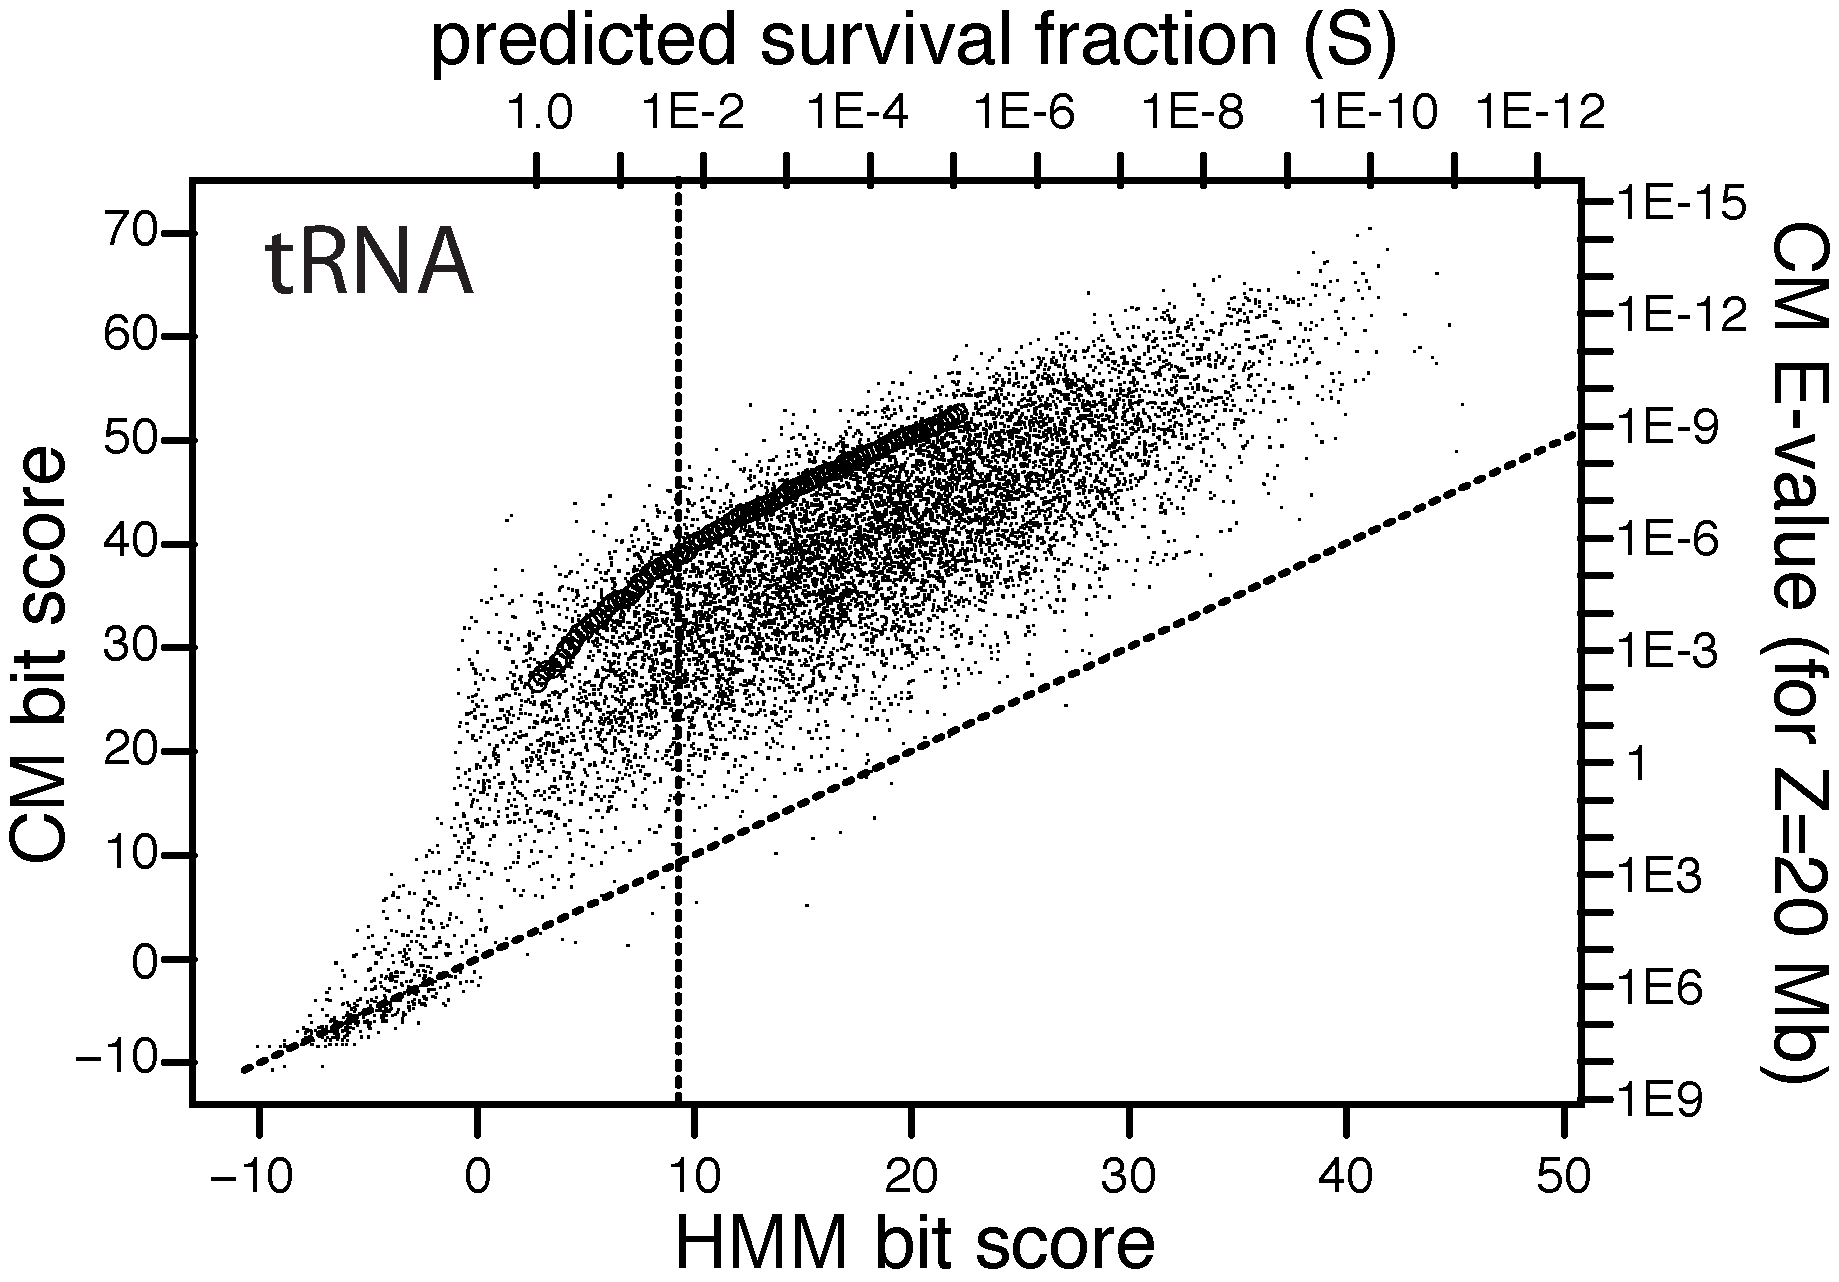
\includegraphics[height=2.5in]{figs/tRNA_fst}
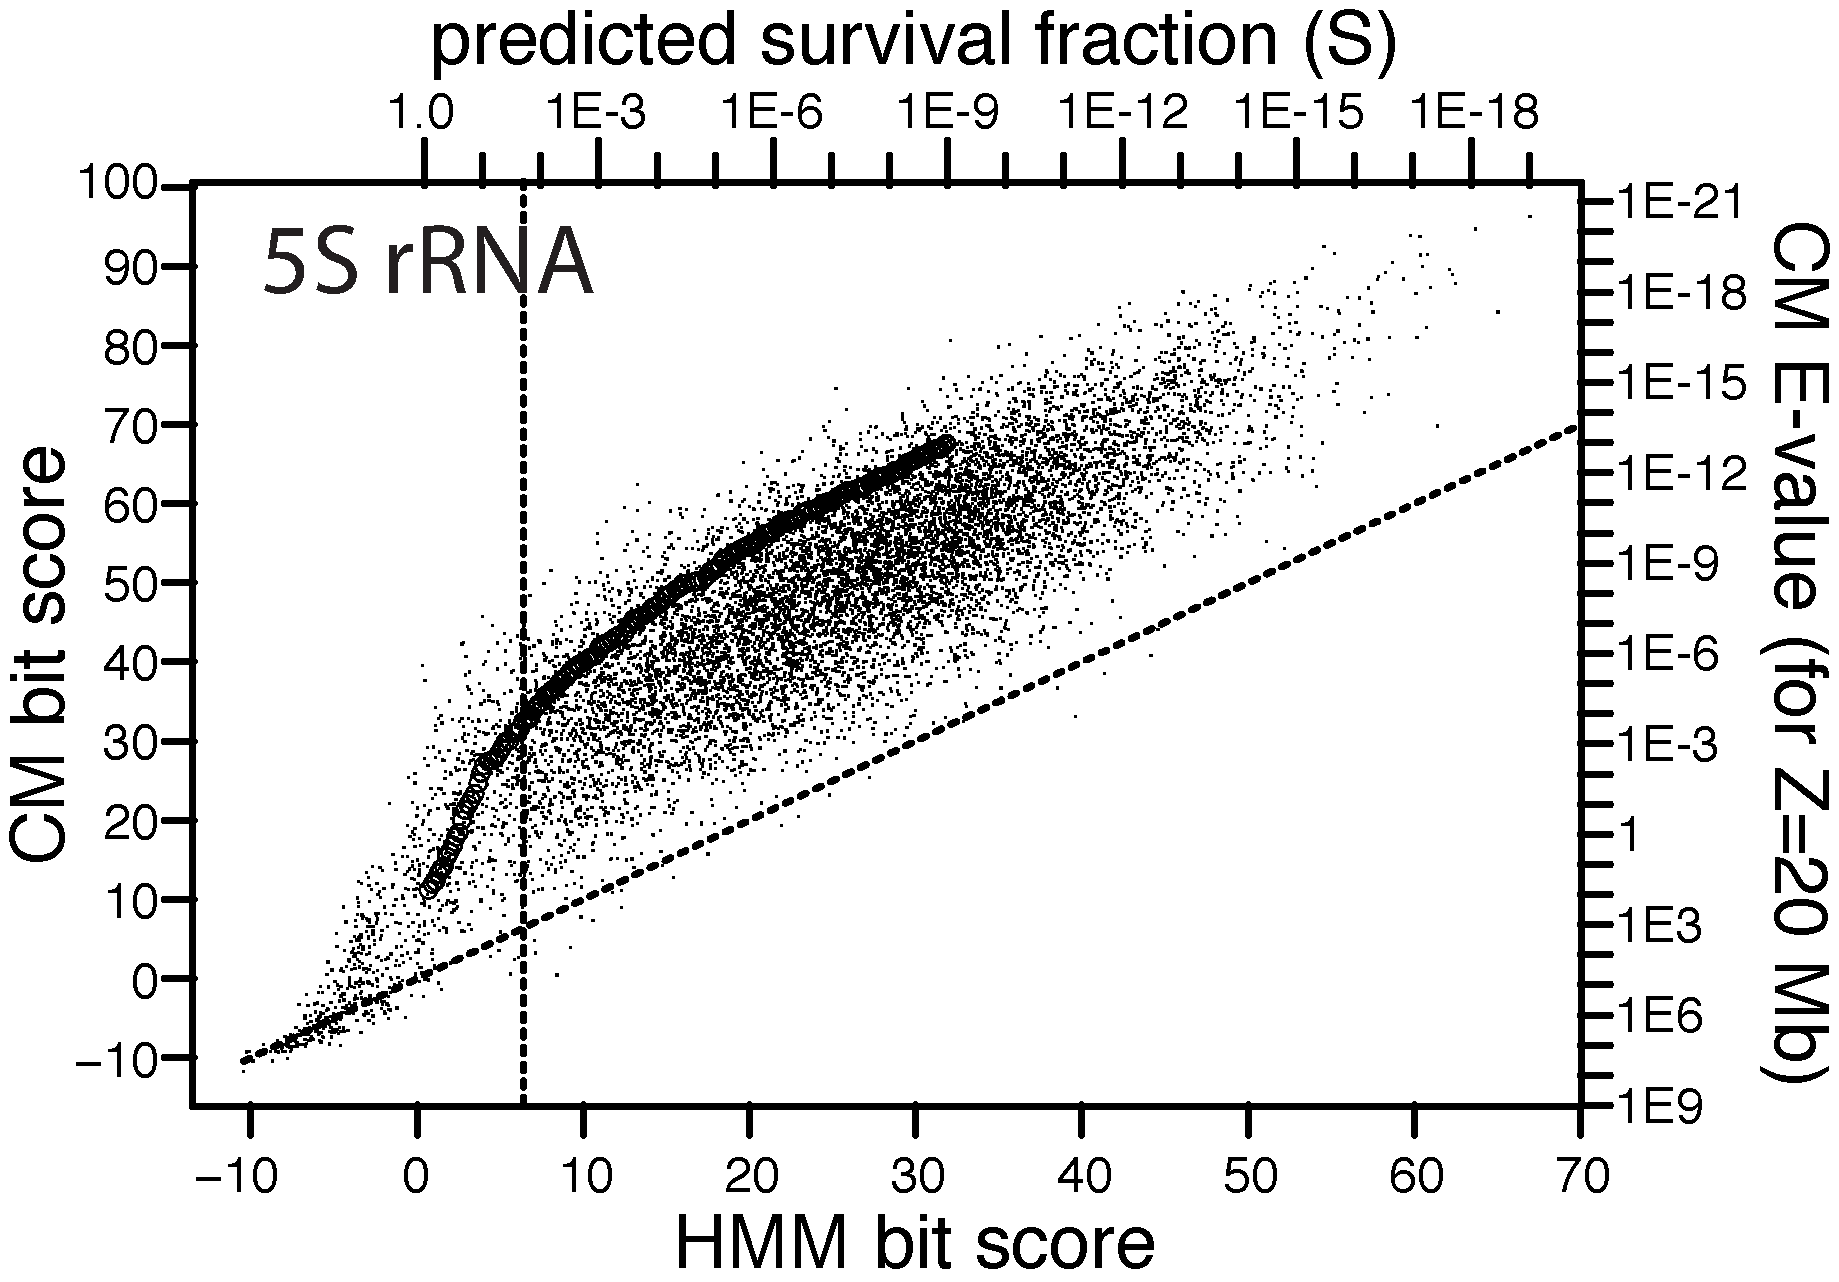
\includegraphics[height=2.5in]{figs/5S_fst}
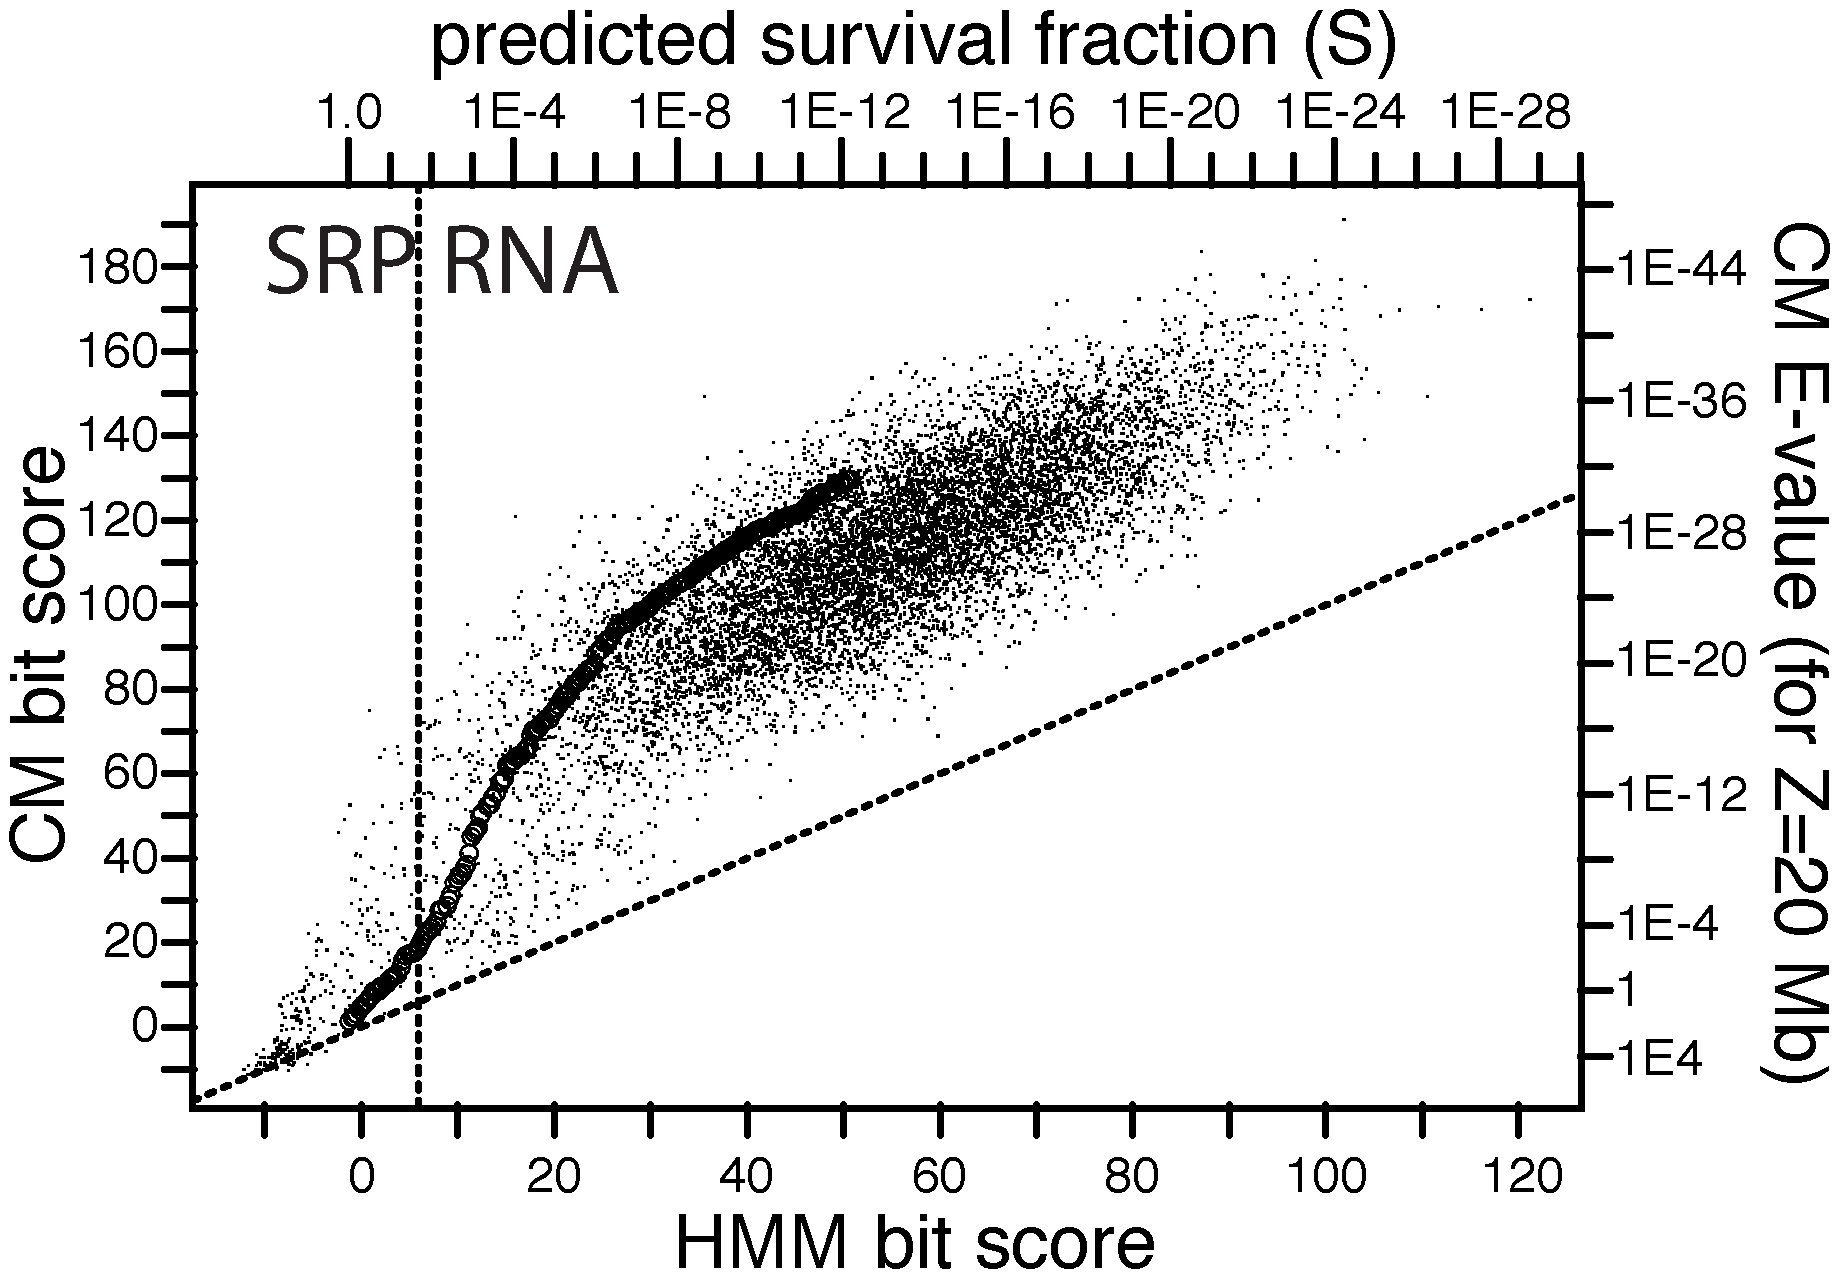
\includegraphics[height=2.5in]{figs/SRP_fst}
%\includegraphics[height=2.5in]{figs/RNaseP_for_ai}
\caption{\textbf{CM Inside scores versus HMM Forward scores during FST calibration.}  
Complete data for the FST calibration with $N=10,000$ and $F=0.99$ of
three anecdotal Rfam 9.1 families: 5S rRNA, tRNA, and RNase P
(RF00001, RF00005, RF00011).  Each sequence is represented as a black
point with x-coordinate equal to it's HMM Forward score, and
y-coordinate equal to it's CM Inside score.  Red circles indicate the
representative set of saved filter survival threshold $T$ and CM
reporting score threshold $C$ pairs saved to the CM file and used to
determine thresholds during searching. The CMs used for sampling and
scoring, and HMMs used for scoring were locally configured.}






\label{Fig:fst}
\end{center}
\end{figure}

\newpage

\begin{figure}
\begin{center}
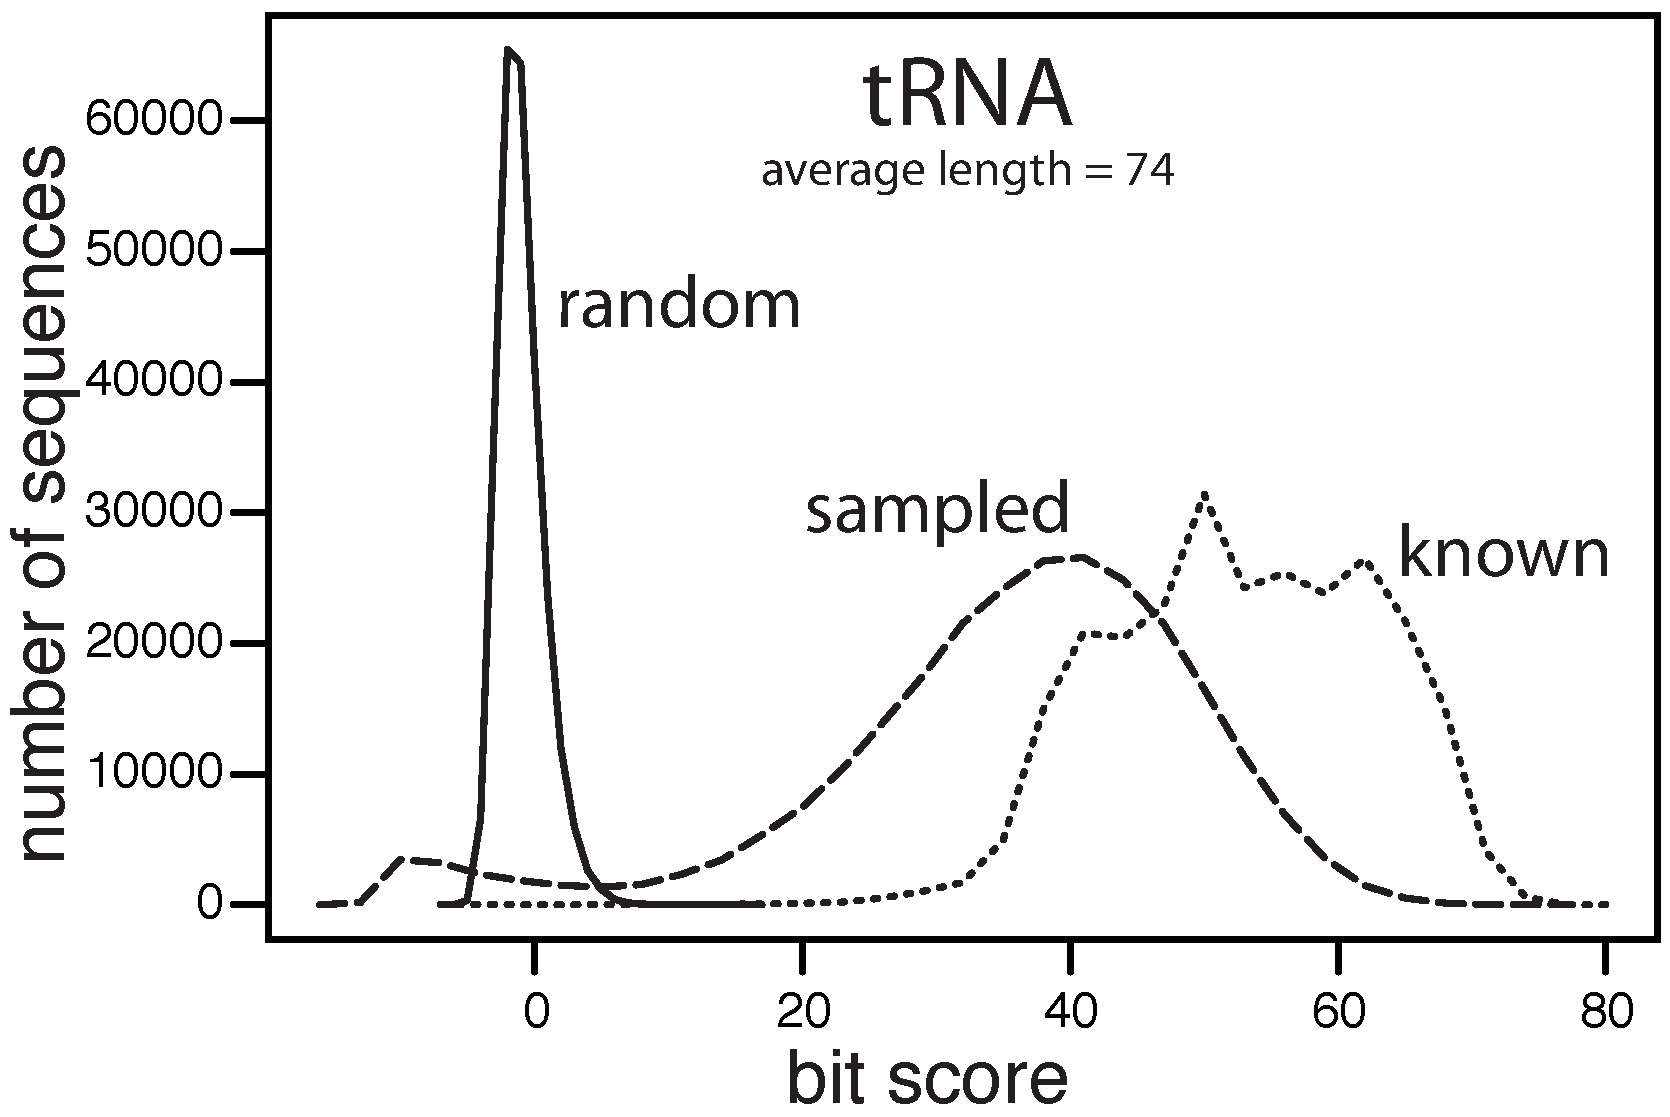
\includegraphics[height=2.1in]{figs/tRNA_sh}

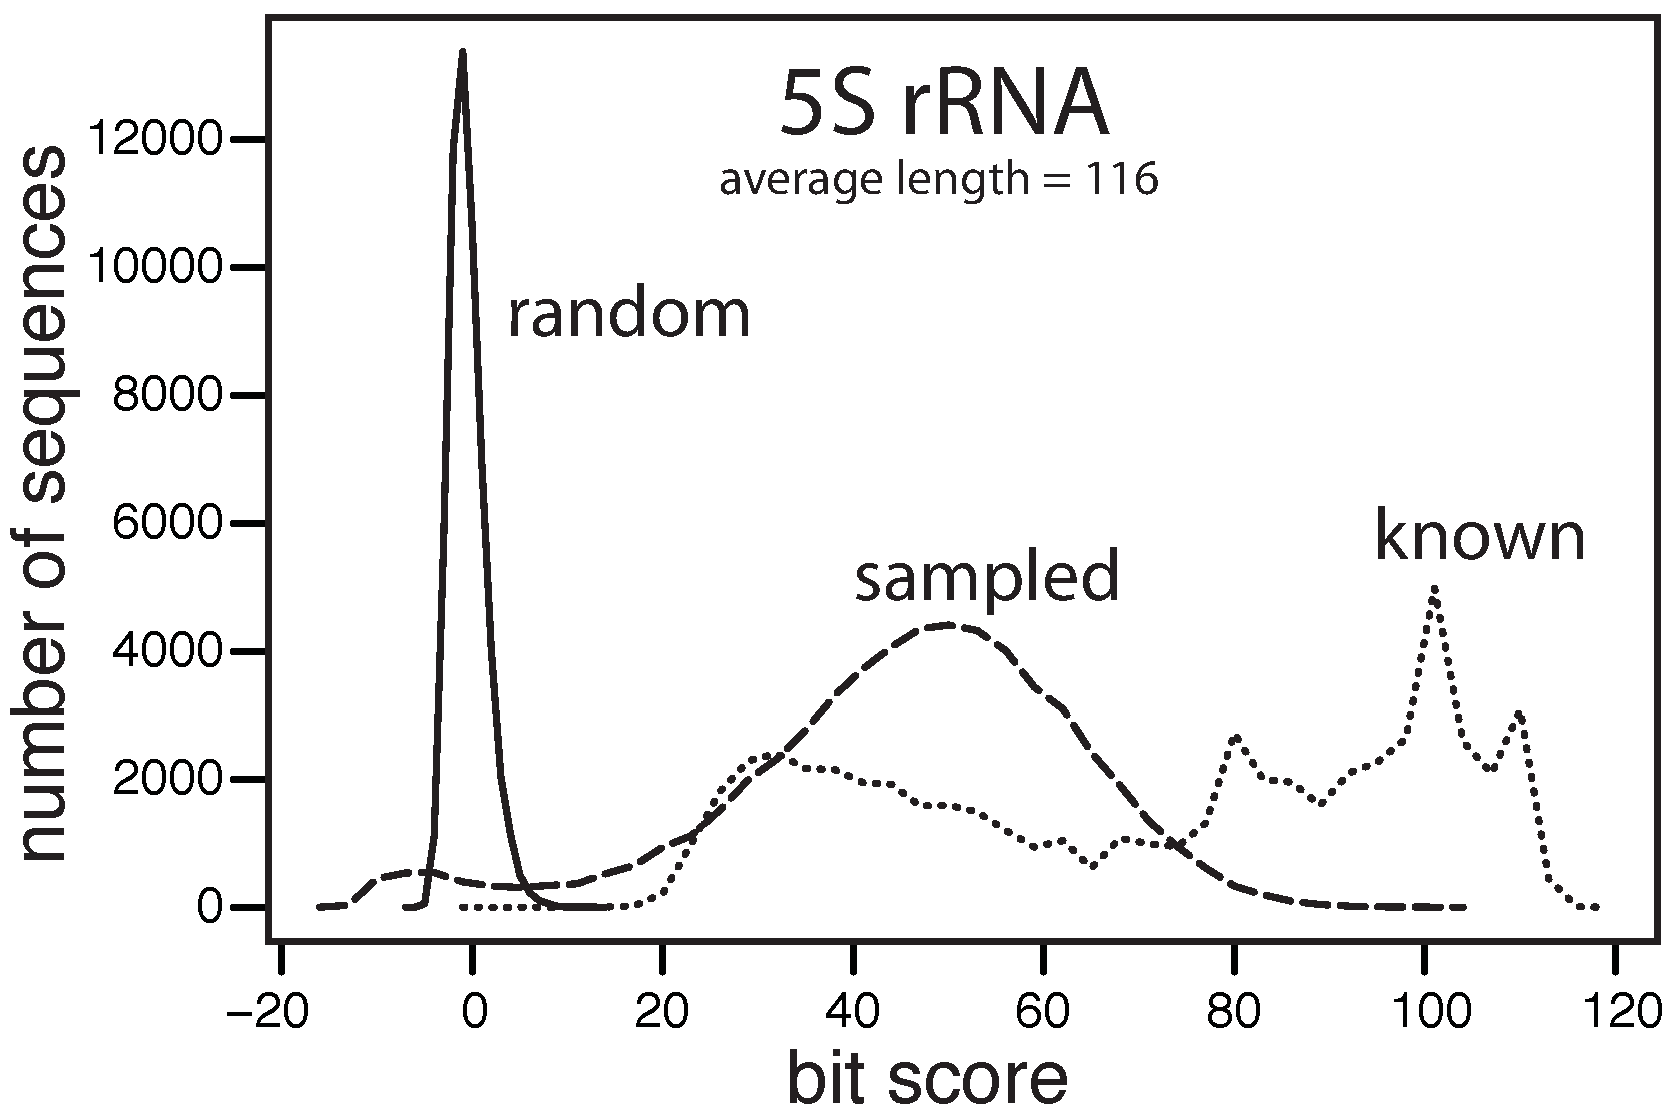
\includegraphics[height=2.1in]{figs/5S_sh}

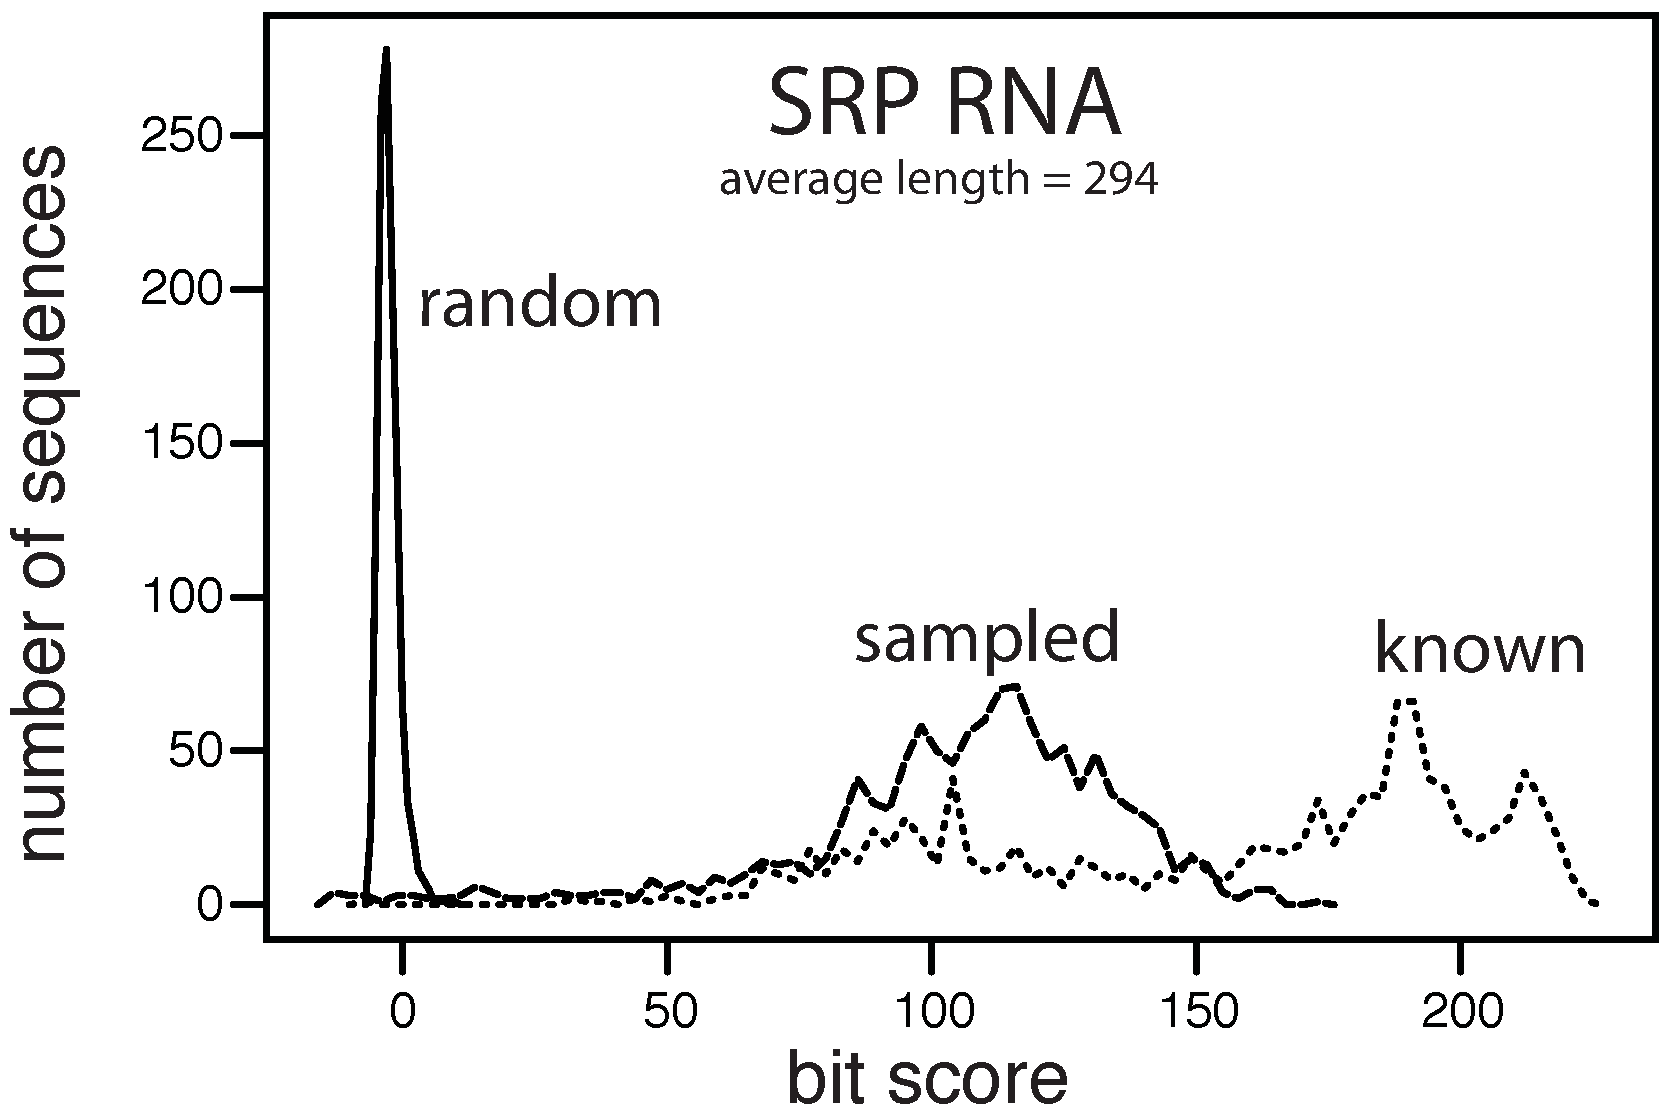
\includegraphics[height=2.1in]{figs/SRP_sh}
\caption{\textbf{CM score histograms of random, known, and sampled
sequences for three RNA families.}  CMs were built from \textsc{Rfam}
9.1 seed alignments using default parameters in \textsc{infernal} 1.01
for three families: tRNA (RF00005), 5S rRNA (RF00001), and SRP RNA
(RF00017).  ``random'' sequences were generated independently for each
family using a single state HMM with equiprobale emission
probabilities ($0.25$) for the four possible RNA bases to be a
specific length $L$, the average length of each family. The
``sampled'' sequences were sampled from locally configured CMs using
the \texttt{cmemit} program of \textsc{infernal} v1.01. The ``known''
sequences are the combination of the ``seed'' and ``full'' sequences
from \textsc{Rfam}. All the sequences were scored using the non-banded
Inside algorithm, and the scores were collated into a histogram of bit
scores. The number of ``random'' and ``sampled'' sequences was set per
family to be equal to the number of ``known'' sequences for that
family: $261,247$ for tRNA, $57,766$ for 5S, and $1187$ for SRP.}






\label{Fig:hists}
\end{center}
\end{figure}

\newpage

\begin{figure}[h]
\centerline{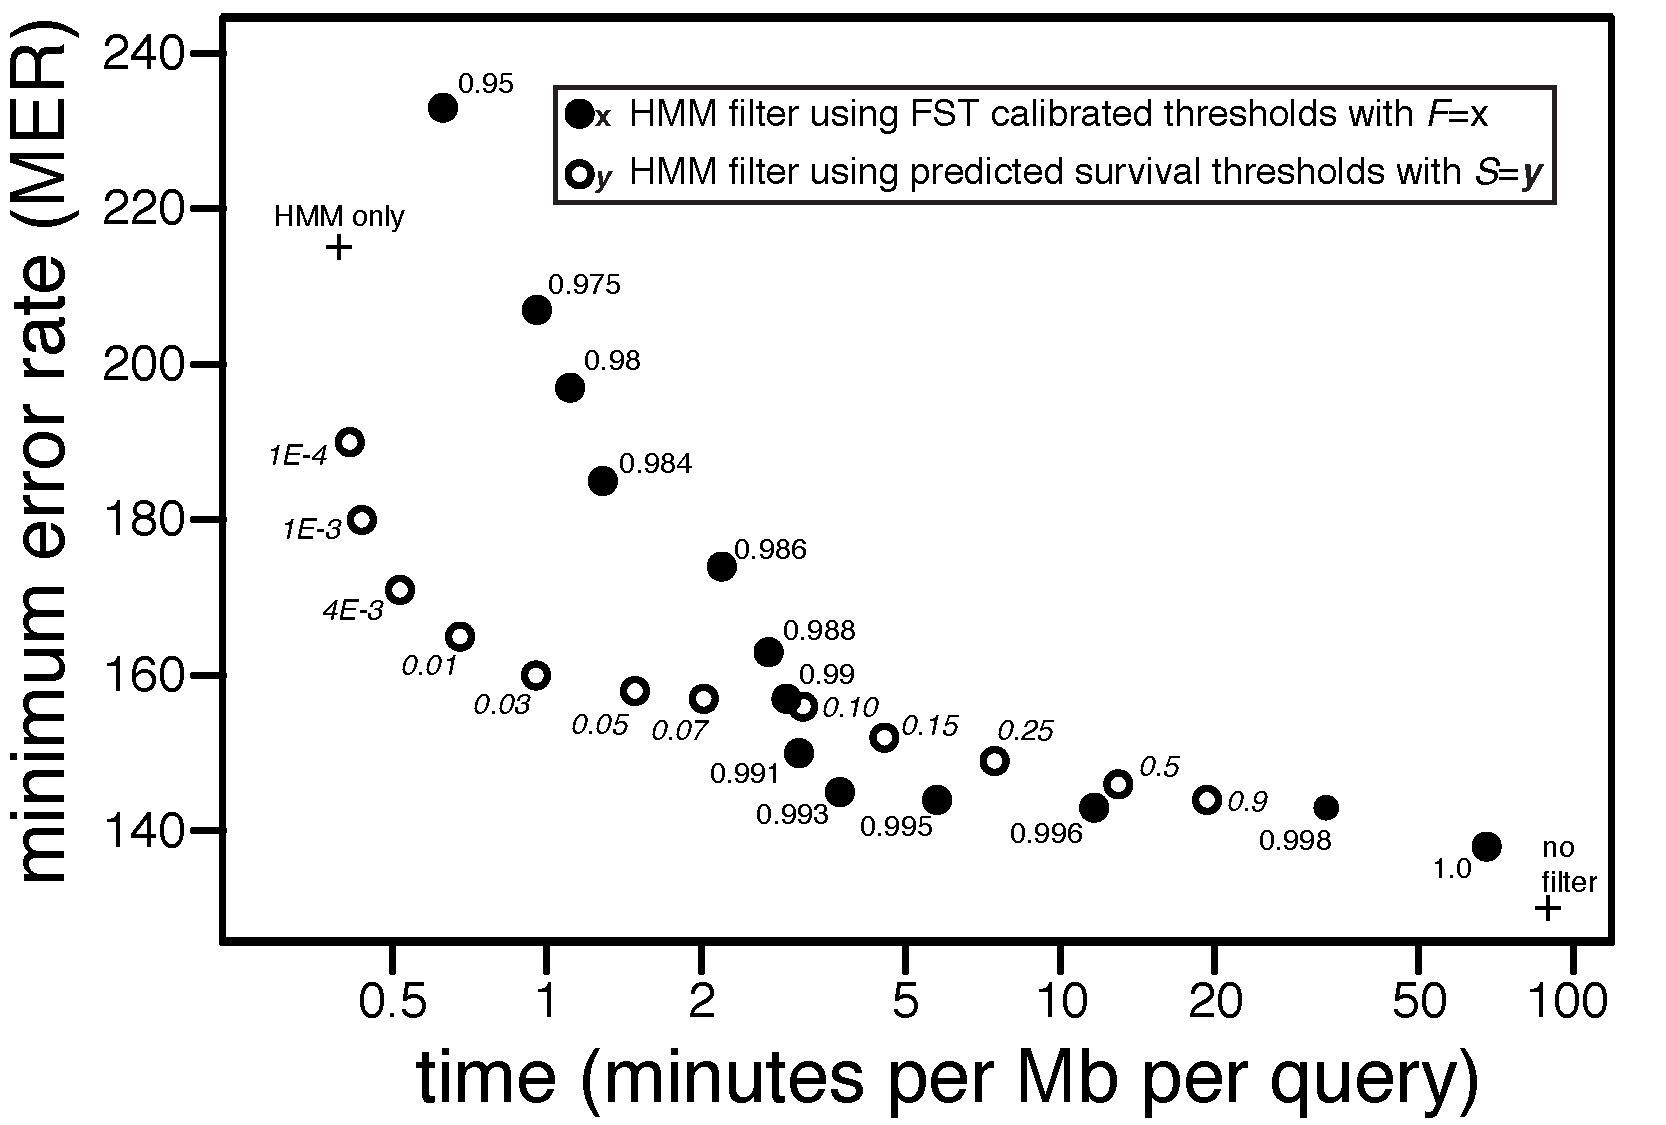
\includegraphics[width=6.4in]{figs/mervtime}}
\caption{\textbf{MER versus time for the benchmark.} 
Solid black points show benchmark performance for HMM filtered
searches using query-dependent FST calibrated filter thresholds with
target sensitivity $F=x$, with $x$ labelled per point.  Open-circle
points show benchmark performance for HMM filtered searches using a
single, query-independent, target survival threshold of $S=y$, with
$y$ labelled per point. There are two additional ``+'' points: ``HMM
only'': HMM Forward algorithm as the final scoring algorithm (with no
filters); ``no filter'' Inside with QDB ($\beta=10^{-15}$) as the
final algorithm. For the FST searches $S_{min} = 0.$. All searches
performed with \textsc{infenral} 1.01. Note that the x-axis is in
log-scale.}









\label{Fig:mervtime}
\end{figure}

\newpage

\begin{figure}
\begin{center}
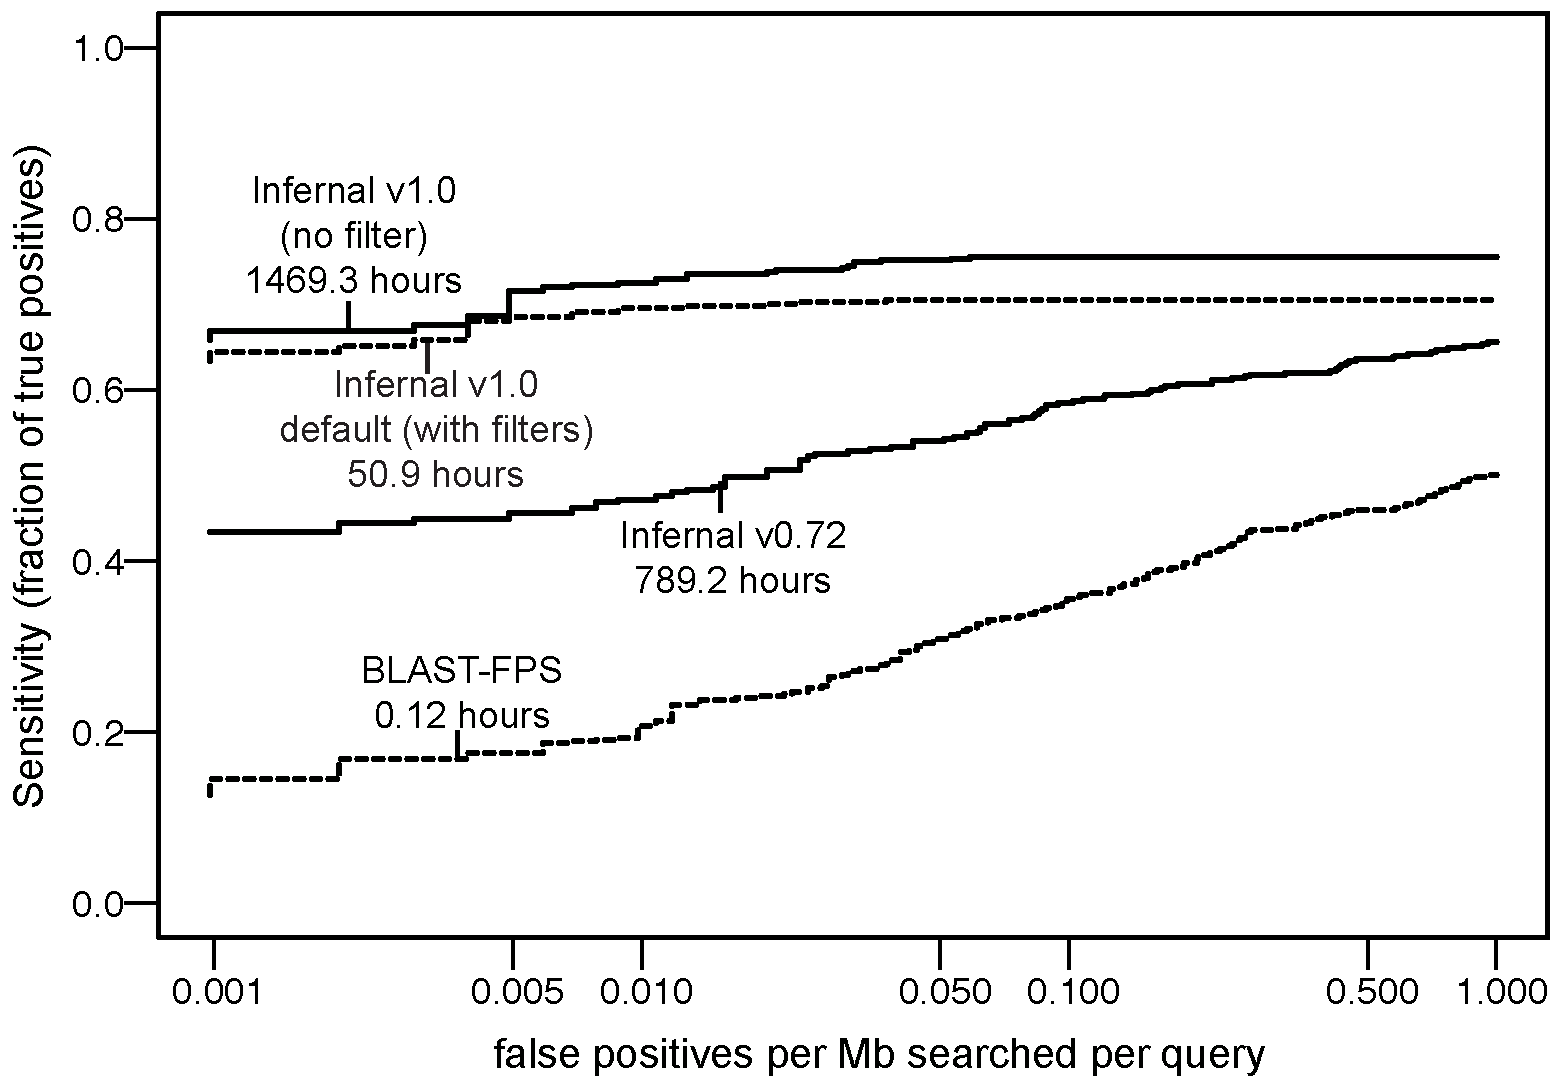
\includegraphics[width=6.4in]{figs/roc}
\caption{\textbf{ROC curves for the benchmark.}  Plots are shown for
\textsc{infernal} 1.01 non-filtered CM searches, default filtered searches, and
HMM only searches, and for \textsc{RaveNnA} 0.2f searches and for
family-pairwise-searches (FPS) with \textsc{blastn}.}






\label{Fig:roc}
\end{center}
\end{figure}

\newpage

\begin{table}
\begin{center}
\scriptsize
%As of EPN, Wed Jan 14 17:06:43 2009
\begin{tabular}{r|r|rr|r|cc|cc|c|c|r} 
  & \multicolumn{4}{c|}{filtering with HMM}  & \multicolumn{2}{c|}{filtering with CM}  & \multicolumn{2}{c|}{post-filtering}& summary & family & \multicolumn{1}{c}{time} \\ % \multicolumn{2}{c}{time} \\ 
  \cline{2-9} 
  & algorithm & FST $F$& $S_{min}$ & target $S$ & algorithm & QDB $\beta$ & algorithm & QDB  $\beta$           & MER     & MER    & (min/Mb/query) \\ \hline %total hours & min/Mb/query \\ \hline
1 & - & -      &    - &    -             & - & -           & Inside    & -                                    & 150     & 115    & 280.60 \\               %4770.2      & 280.6 \\
2 & - & -      &    - &    -             & - & -           & CYK       & -                                    & 156     & 133    & 102.16 \\ %1736.7      & 102.2 \\
3 & - & -      &    - &    -             & - & -           & Inside    & $10^{-15}$                           & 130     & 109    &  89.13\\ %1515.2      & 89.1 \\
%4 & - & -      &    - &    -             & - & -           & CYK       & $10^{-7}$                            & 156     & 127    &  15.82\\ %269.0       & 15.8 \\
4 & - & -      &    - &    -             & - & -           & CYK       & $10^{-15}$                           & 153     & 130    &  30.60\\ %520.2       & 30.6 \\
5 & - & -      &    - &    -             & - & -             & CYK       & $10^{-10}$                          & 154     & 132    &  21.97\\ %373.43      
& & & & & & & & & & & \\
6 & - & -      &    - &    -             & CYK & $10^{-13}$   & Inside    & $10^{-15}$                         & 131     & 114    &  30.08\\ %511.4       
7 & - & -      &    - &    -             & CYK & $10^{-10}$   & Inside    & $10^{-15}$                         & 130     & 114    &  24.24\\ %296.2       & 17.4 \\ 
8 & - & -      &    - &    -             & CYK & $10^{-7}$   & Inside    & $10^{-15}$                         & 134     & 118    &  17.42\\ %296.2       & 17.4 \\ 
9 & - & -      &    - &    -             & CYK & $10^{-4}$   & Inside    & $10^{-15}$                         & 142     & 127    &  10.18\\ %296.2       & 17.4 \\ 
& & & & & & & & & & & \\
%\hline% & & & & & & & & & & \\
%9 & Forward & - & - & 0.01             & - & -           & Inside    & $10^{-15}$                          & 165     & 153    &  0.68\\ %11.5      & 0.7 \\
%9 & Forward & - & - & 0.01             & - & -           & Inside    & $10^{-15}$                          & 165     & 153    &  0.68\\ %11.5      & 0.7 \\
10 & Forward & - & - & 0.02             & - & -           & Inside    & $10^{-15}$                          & 160     & 149    &  0.95\\ %16.2      & 16.2 \\
11 & Forward & - & - & 0.10             & - & -           & Inside    & $10^{-15}$                          & 156     & 142    &  3.16 \\ %53.7      & 3.2 \\
12 & Forward & - & - & 0.25             & - & -           & Inside    & $10^{-15}$                          & 149     & 131    &  7.46 \\ %126.8     & 7.5 \\
& & & & & & & & & & & \\
%\hline% & & & & & & & & & & \\
13& Forward & $0.993$& -    & -              & - & -           & Inside    & $10^{-15}$                       & 145     & 135    &  3.73 \\ % 63.4     & 3.8 \\
%\hline%& & & & & & & & & & \\
%11& Forward & $0.993$& 0.0001 & -            & - & -           & Inside    & $10^{-15}$                      & 145     & 135    &  3.73 \\ % 63.4     & 3.8 \\
14& Forward & $0.993$& 0.01 & -              & - & -           & Inside    & $10^{-15}$                       & 144     & 134    &  3.84 \\ % 65.3     & 3.8 \\
15& Forward & $0.993$& 0.02 & -              & - & -           & Inside    & $10^{-15}$                       & 143     & 133    &  3.99 \\ % 67.8     & 4.0 \\
16& Forward & $0.993$& 0.10 & -              & - & -           & Inside    & $10^{-15}$                       & 143     & 132    &  5.64 \\ % 95.9     & 5.6 \\
& & & & & & & & & & & \\
%\hline% & & & & & & & & & & \\
%14& Forward & - & - & 0.01           & CYK & $10^{-7}$   & Inside    & $10^{-15}$                         & 167     & 161    &  0.58 \\ %  9.9     & 0.6 \\
17& Forward & - & - & 0.02           & CYK & $10^{-10}$   & Inside    & $10^{-10}$                          & 161     & 154    &  0.68 \\ %  11.6    & 0.7 \\ \hline
%17& Forward & $0.993$& 0.02 & -           & CYK & $10^{-7}$   & Inside    & $10^{-15}$                     & 145     & 136    &  1.12 \\ % 19.0    & 1.1 \\ \hline
18& Forward & $0.993$& 0.02 & -           & CYK & $10^{-10}$  & Inside    & $10^{-15}$                     & 143     & 134    &  1.26 \\ % 21.6    & 1.1 \\ \hline
& & & & & & & & & & & \\
19& -       & -      &    - & -           &   - &       -     & HMM Forward & -                            & 214     & 204    & 0.39  \\ %6.71 & 0.4 \\

%11 & FST; $0.995$& $\beta=10^{-7}$ & Inside $\beta=10^{-15}$ & 146    & 135    & 50.9 \\
%12 & $E=10000$     & none            & Inside $\beta=10^{-15}$ & 151    & 140    & 119.0 \\
%6 & $E=2500$      & none            & Inside; $\beta=10^{-15}$ & 159     & 151    & 34.1 \\
%7 & $E=5000$         & none         & Inside; $\beta=10^{-15}$ & 155     & 145    & 64.3 \\
\end{tabular}


%%%%%%%%%%%%%%%%%%%%%%%%%%%%%%%%%%%%%%%%%%%%%%%%%%%%%%%%%%%%%%%%%%%%%%%
\begin{comment}
%%%%%%%%%%%%%%%%%%%%%%%%%%%%%%%%%%%%%%%%%%%%%%%%%%%%%%%%%%%%%%%%%%%%%%%
\begin{tabular}{cccccr} 
                        &               &               & summary & family-specific &          \\ 
program                 & HMM filtered? & CYK filtered? & MER     & MER             & time (h) \\ \hline
\textsc{blastn}         & -             & -             & 357     & 253             & 0.1 \\ %0.12 \\
\textsc{infernal} 0.72  & no            & no            & 240     & 177             & 789.2 \\
\textsc{infernal} 1.0   & no            & no            & 130     & 112             & 1477.2 \\
\textsc{infernal} 1.0   & no            & yes           & 134     & 118             & 296.2 \\
\textsc{infernal} 1.0   & yes           & no            & 143     & 131             & 257.9 \\
\textsc{infernal} 1.0   & yes           & yes           & 146     & 135             &  50.9 \\
\end{tabular}
%%%%%%%%%%%%%%%%%%%%%%%%%%%%%%%%%%%%%%%%%%%%%%%%%%%%%%%%%%%%%%%%%%%%%%%
\end{comment}

\begin{comment}
\begin{tabular}{ccccccr} 
                        & HMM           & CYK             & final                   & summary & family-specific &          \\ 
program                 & filter        & filter          & round                   & MER     & MER             & time (h) \\ \hline
\textsc{blastn}         & -             & -               & -                       & 357     & 253             & 0.1 \\ %0.12 \\
%\textsc{infernal} 0.72  & no           & no              & CYK                     & 240     & 177             & 789.2 \\
\textsc{infernal} 1.0   & none          & none            & Inside no QDBs          & ?       & ?               & ? \\
\textsc{infernal} 1.0   & none          & none            & Inside $\beta=10^{-15}$ & 130     & 112             & 1477.2 \\
\textsc{infernal} 1.0   & none          & none            & CYK    $\beta=10^{-7}$  & ?       & ?               & 296.2 \\
\textsc{infernal} 1.0   & none          & $\beta=10^{-7}$ & Inside $\beta=10^{-15}$ & 134     & 118             & 296.2 \\
\textsc{infernal} 1.0   & FST           & none            & Inside $\beta=10^{-15}$ & 143     & 131             & 257.9 \\
\textsc{infernal} 1.0   & FST           & $\beta=10^{-7}$ & Inside $\beta=10^{-15}$ & 146     & 135             &  50.9 \\

\end{tabular}
\end{comment}

\begin{comment}
%%%%%%%%%%%%%%%%%%%%%%%%%%%%%%%%%%%%%%%%%%%%%%%%%%%%%%%%%%%%%%%%%%
pre-EPN, Wed Jan 14 17:06:29 2009
\begin{tabular}{r|c|c|c|c|c|r} 
  & HMM           & CYK             & final                    & summary & family &          \\ 
  & filter        & filter          & round                    & MER     & MER    & time (h) \\ \hline
1 & none          & none            & Inside; no QDBs          & 150     & 115    & 4770.2 \\
2 & none          & none            & CYK; no QDBs             & 156     & 133    & 1736.7 \\
3 & none          & none            & Inside; $\beta=10^{-15}$ & 130     & 112    & 1477.2 \\
4 & none          & none            & CYK;    $\beta=10^{-7}$  & 156     & 133    & 267.4 \\
5 & none          & $\beta=10^{-7}$ & Inside; $\beta=10^{-15}$ & 134     & 118    & 296.2 \\
%6 & FST; $F=0.995$& none            & Inside $\beta=10^{-15}$ & 143     & 131    & 257.9 \\
7 & $E=25000$     & none            & Inside; $\beta=10^{-15}$ & 147     & 134    & 219.4 \\
6 & $E=3500$      & none            & Inside; $\beta=10^{-15}$ & 157     & 147    & 49.7 \\
8 & FST; $F=0.99 $& none           & Inside; $\beta=10^{-15}$  & 147     & 137    & 51.4 \\
9 & FST; $F=0.99 $& $\beta=10^{-7}$& Inside; $\beta=10^{-15}$ & 148     & 139    & 16.1 \\
%11 & FST; $F=0.995$& $\beta=10^{-7}$ & Inside $\beta=10^{-15}$ & 146    & 135    & 50.9 \\
%12 & $E=10000$     & none            & Inside $\beta=10^{-15}$ & 151    & 140    & 119.0 \\
%6 & $E=2500$      & none            & Inside; $\beta=10^{-15}$ & 159     & 151    & 34.1 \\
%7 & $E=5000$         & none         & Inside; $\beta=10^{-15}$ & 155     & 145    & 64.3 \\
\end{tabular}
\end{comment}
%%%%%%%%%%%%%%%%%%%%%%%%%%%%%%%%%%%%%%%%%%%%%%%%%%%%%%%%%%%%%%%%%%

\normalsize
\end{center}
\caption{\textbf{Benchmark MER and timing statistics for different
search strategies.}  
Each search strategy is defined by the algorithms and parameters used
by zero, one or two filtering stages and a final post-filtering
stage. Under ``filtering with HMM'': ``algorithm'' lists if an HMM
filter is applied first (``Forward''), or not at all (``-''); ``FST
$F$'' lists the target sensitivity $F$ used for FST threshold
calibration, or ``-'' if FST was not used; ``$S_{min}$'' 
is the minimum predicted survival fractions used to set filter
thresholds (potentially overriding the FST calibrated thresholds);
``target $S$'' shows the single, target predicted survival fraction
used for all modles in non-FST HMM filtering strategies.
Under ``filtering with CM'': ``algorithm'' lists if a CM ``CYK''
filter is applied (only on the surviving subsequences from the HMM
filter if one was used) or not at all (``-''), and ``QDB $\beta$''
lists the tail loss probability used to calculate bands for the
algorithm.  Under ``post-filtering'': ``algorithm'' lists the main
algorithm used for scoring subsequences that survive the $<=2$
filtering stages; ``QDB $\beta$'' lists the tail loss probability for
the band calculation for the main algorithm.
The sensitivity and specificity of each strategy is summarized by
``summary MER'' and ``family MER'' as explained in the text. Lower
MERs are better.  ``min/Mb/query'' list minutes per Mb (1,000,000
residues) of search space per query model used to search. The
benchmark contains 51 query models and 20 Mb of search space (both
strands of the 10 Mb pseudogenome) as explained in the text.}

\begin{comment}
%ALTERNATE MIDDLE SECTION
For the ``filtering with CM'' and ``post-filtering'' sections:
``algorithm'' lists the CM algorithm used on the survival fraction
from the HMM filter (if one was used) for either filtering (under
``filtering with CM'') or for final scoring of sequences that survived
up to two filters (``post-filtering''); ``QDB $\beta$'' lists the tail
loss probability used to define bands for the CM algorithm
\citep{NawrockiEddy07}.
\end{comment}

\label{Tab:merlist}
\end{table}


\begin{table}
\begin{center}
\scriptsize
\begin{tabular}{rllrrr|rr|rr|rr} 
\multicolumn{3}{c}{Predicted survival fraction ($S$)}&& & non-     & \multicolumn{2}{c|}{FST HMM filtering}           & \multicolumn{2}{c|}{FST HMM filtering}             & \multicolumn{2}{c}{Non-FST HMM filtering} \\
\multicolumn{3}{c}{range for FST HMM filter}         &\#&\#& filtered & \multicolumn{2}{c|}{($F=0.993$, no $S_{min}$)}   & \multicolumn{2}{c|}{($F=0.993$, $S_{min}=0.02$)}   & \multicolumn{2}{c}{single threshold ($S=0.02$)} \\ \cline{7-12}
\multicolumn{3}{c}{($F=0.993$, no $S_{min}$)}        & query & test & \# found &actual $F$& speedup                               & actual $F$& speedup                                &actual $F$& speedup            \\\hline                    
(no filter) & $S$ &$=1.0$& 2      &  52    & 43       & 1.000    &   1.0                                 & 1.000    &   1.0                                   & 0.581    &  70.9 \\                               
$1.0 >$& $S$ &$>= 0.1$& 11     &  98    & 76       & 0.987    &  10.6                                 & 0.987    &  10.6                                   & 0.974    &  79.3 \\                               
$0.1 >$& $S$ &$>=1e-2$& 17     & 165    & 135      & 0.919    &  52.8                                 & 0.919    &  51.0                                   & 0.911    &  88.6 \\                               
$1e-2>$& $S$ &$>=1e-3$&  8     &  54    & 48       & 0.854    & 150.8                                 & 0.854    &  72.1                                   & 0.854    &  80.9 \\                               
$1e-3>$& $S$ &$>=1e-4$&  7     &  53    & 31       & 0.807    & 185.0                                 & 0.871    & 103.0                                   & 0.871    & 121.2 \\                               
$1e-4>$& $S$ &$>=1e-5$&  4     &   6    & 4        & 1.000    &  90.4                                 & 1.000    &  57.8                                   & 1.000    &  67.6 \\                                
$1e-5>$& $S$ &$>  0  $&  2     &  22    & 4        & 0.750    & 265.5                                 & 0.750    & 121.6                                   & 0.750    & 143.6 \\ \hline
       & all &        & 51     & 450    & 341      & 0.924    &  23.9                                 & 0.930    &  22.3                                   & 0.871    &  93.4 \\                               
\end{tabular}

\normalsize
\end{center}
\caption{\textbf{Comparison of filter sensitivity and benchmark 
      acceleration for queries with different FST predicted filter
      survival fractions.}
  The 51 query benchmark families were
  categorized based on the predicted survival fraction $S$ of a FST
  filtered HMM benchmark search with final reporting threshold
  $E=1$. FST was performed with $F=0.993$ and no $S_{min}$
  value. Column 1 lists the survival fraction category; the first row
  ``no filter $S=1.0$'' corresponds to queries for which FST indicates
  $S>=1.0$ so the HMM filter is turned off. The next three columns
  list the number of query families (``\# query''), total number of
  test sequences (``\# test''), and number of the test sequences that
  the main algorithm scores with $E<=1$ (``non-filtered \#
  found''). The remaining six columns compare three filtering
  strategies: FST HMM filtering using $F=0.993$ and no $S_{min}$ value
  (this is row 10 in Table~1), FST HMM filtering with $F=0.993$ and no
  $S_{min}=0.02$ (row 12 in Table~1), and non-FST filtering setting
  thresholds that give a predicted $S=0.02$ (row 14 in Table~1). For
  each strategy: ``actual $F$'' lists the filter sensitivity per
  category, the fraction of the test sequences the main algorithm
  scores $E<=1$ that also pass the filter score threshold and survive
  the filter; ``speedup'' lists the per-category acceleration of a
  filtered search versus a non-filtered search in the benchmark.  Only
  HMM filters were used (no CYK filters). The main algorithm used was
  Inside with QDBs calculated with $\beta=10^{-15}$.}






\label{Tab:survcat}
\end{table}


\begin{table}
\begin{center}
\scriptsize
\begin{tabular}{lrr|rr|rr|rr} 
\multicolumn{1}{c}{main algorithm E-value}  & corresponding       & non-     & \multicolumn{2}{c|}{FST HMM filtering}         & \multicolumn{2}{c|}{FST HMM filtering}           & \multicolumn{2}{c}{Non-FST HMM filtering} \\
\multicolumn{1}{c}{reporting threshold}     & database size for   & filtered & \multicolumn{2}{c|}{($F=0.993$, no $S_{min}$)} & \multicolumn{2}{c|}{($F=0.993$, $S_{min}=0.02$)} & \multicolumn{2}{c}{single threshold ($S=0.02$)} \\ \cline{4-9}
\multicolumn{1}{c}{(database size = 20 Mb)} & $E=1$ threshold     & \# found & actual $F$& speedup                            & actual $F$& speedup                              &actual $F$& speedup            \\\hline                    
  $E=1e-5$                                    &             2 Tb    & 250      & 0.880 &  108.5                             & 0.984     &  66.3                                & 0.980    & 89.0 \\
  $E=1e-4$                                    &           200 Gb    & 268      & 0.892 &   91.9                             & 0.974     &  60.8                                & 0.966    & 89.0 \\
  $E=1e-3$                                    &            20 Gb    & 285      & 0.902 &   73.1                             & 0.965     &  53.6                                & 0.940    & 89.0 \\
  $E=1e-2$                                    &             2 Gb    & 298      & 0.920 &   38.2                             & 0.960     &  32.5                                & 0.920    & 89.0 \\
  $E=1e-1$                                    &           200 Mb    & 324      & 0.926 &   29.2                             & 0.954     &  26.1                                & 0.904    & 89.0 \\
  $E=1$                                    &            20 Mb    & 341      & 0.924 &   23.9                             & 0.930     &  22.3                                & 0.871    & 89.0 \\
  $E=10$                                    &             2 Mb    & 355      & 0.913 &   15.4                             & 0.916     &  14.8                                & 0.851    & 89.0 \\
  $E=100$                                    &           200 Kb    & 368      & 0.910 &    4.9                             & 0.913     &   4.8                                & 0.834    & 89.0 \\
  $E=1000$                                    &            20 Kb    & 391      & 0.910 &    2.9                             & 0.910     &   2.9                                & 0.800    & 89.0 \\
\end{tabular}


%original data from ../evaluate_F_dir/ins.l.Smin0.data and ../evaluate_F_dir/ins.l.Sminp02.data and 
\begin{comment}
ins.l.FST.Ep00001.surv.Smin0.tbl  &   89.02    0.82  &  0.8800  &   108.518&   0  &       -  &         -&   2  &  0.9444  &     8.257&   4  &  1.0000  &    66.591&   9  &  0.8889  &   113.419&   5  &  1.0000  &   202.271&   7  &  1.0000  &   200.918&  24  &  0.6977  &   184.873
ins.l.FST.Ep0001.surv.Smin0.tbl   &   89.02    0.97  &  0.8918  &    91.935&   0  &       -  &         -&   3  &  0.8846  &     7.060&   6  &  0.9804  &    61.185&   9  &  0.9200  &   128.286&   6  &  0.9861  &   189.658&   8  &  1.0000  &   173.949&  19  &  0.7471  &   191.215
ins.l.FST.Ep001.surv.Smin0.tbl    &   89.02    1.22  &  0.9018  &    73.092&   0  &       -  &         -&   4  &  0.9149  &     5.841&   9  &  1.0000  &    53.761&   9  &  0.7895  &   133.026&   6  &  0.9692  &   166.481&   9  &  1.0000  &   182.461&  14  &  0.7778  &   192.564
ins.l.FST.Ep01.surv.Smin0.tbl     &   89.02    2.33  &  0.9195  &    38.226&   1  &  1.0000  &         -&   3  &  0.9615  &     6.320&  14  &  0.9375  &    39.080&  11  &  0.9659  &   153.867&   4  &  0.8889  &   192.602&   7  &  0.8929  &   147.782&  11  &  0.7966  &   203.721
ins.l.FST.Ep1.surv.Smin0.tbl      &   89.02    3.05  &  0.9259  &    29.218&   2  &  1.0000  &         -&   8  &  1.0000  &    13.292&  12  &  0.8718  &    49.803&  10  &  0.9464  &   137.499&   5  &  0.8889  &   200.440&  11  &  0.8226  &   176.429&   3  &  0.8000  &   225.590
ins.l.FST.E1.surv.Smin0.tbl       &   89.02    3.73  &  0.9238  &    23.890&   2  &  1.0000  &         -&  11  &  0.9868  &    10.578&  17  &  0.9185  &    52.837&   8  &  0.8542  &   150.786&   7  &  0.8065  &   185.021&   4  &  1.0000  &    90.526&   2  &  0.7500  &   265.514
ins.l.FST.E10.surv.Smin0.tbl      &   89.02    5.80  &  0.9127  &    15.354&   2  &  1.0000  &         -&  21  &  0.9697  &     8.139&  12  &  0.8647  &    37.931&   9  &  0.7714  &   171.592&   5  &  1.0000  &    94.120&   1  &  1.0000  &   146.122&   1  &  0.6667  &   387.492
ins.l.FST.E100.surv.Smin0.tbl     &   89.02   18.31  &  0.9103  &     4.861&   6  &  1.0000  &         -&  25  &  0.9075  &     6.655&  11  &  0.7561  &    65.373&   8  &  0.7222  &   124.017&   0  &       -  &         -&   1  &  0.5000  &   387.447&   0  &       -  &         -
ins.l.FST.E1000.surv.Smin0.tbl    &   89.02   30.76  &  0.9105  &     2.894&  12  &  1.0000  &         -&  29  &  0.8679  &     5.647&  10  &  0.5758  &    47.588&   0  &       -  &         -&   0  &       -  &         -&   0  &       -  &         -&   0  &       -  &         -

ins.l.Sp02.Ep00001.surv.Smin0.tbl &   89.02    0.95  &  0.9800  &    93.379&   2  &  0.8889  &         -&  11  &  1.0000  &    79.333&  17  &  0.9748  &    88.642&   8  &  1.0000  &    80.856&   7  &  1.0000  &   121.168&   4  &  0.0000  &    67.636&   2  &  1.0000  &   143.586
ins.l.Sp02.Ep0001.surv.Smin0.tbl  &   89.02    0.95  &  0.9664  &    93.379&   2  &  0.7826  &         -&  11  &  1.0000  &    79.333&  17  &  0.9752  &    88.642&   8  &  1.0000  &    80.856&   7  &  0.9600  &   121.168&   4  &  0.0000  &    67.636&   2  &  1.0000  &   143.586
ins.l.Sp02.Ep001.surv.Smin0.tbl   &   89.02    0.95  &  0.9404  &    93.379&   2  &  0.6552  &         -&  11  &  1.0000  &    79.333&  17  &  0.9600  &    88.642&   8  &  1.0000  &    80.856&   7  &  0.9259  &   121.168&   4  &  0.0000  &    67.636&   2  &  1.0000  &   143.586
ins.l.Sp02.Ep01.surv.Smin0.tbl    &   89.02    0.95  &  0.9195  &    93.379&   2  &  0.6250  &         -&  11  &  1.0000  &    79.333&  17  &  0.9457  &    88.642&   8  &  0.9714  &    80.856&   7  &  0.8621  &   121.168&   4  &  1.0000  &    67.636&   2  &  1.0000  &   143.586
ins.l.Sp02.Ep1.surv.Smin0.tbl     &   89.02    0.95  &  0.9043  &    93.379&   2  &  0.6154  &         -&  11  &  1.0000  &    79.333&  17  &  0.9318  &    88.642&   8  &  0.9524  &    80.856&   7  &  0.8710  &   121.168&   4  &  1.0000  &    67.636&   2  &  0.7500  &   143.586
ins.l.Sp02.E1.surv.Smin0.tbl      &   89.02    0.95  &  0.8710  &    93.379&   2  &  0.5814  &         -&  11  &  0.9737  &    79.333&  17  &  0.9111  &    88.642&   8  &  0.8542  &    80.856&   7  &  0.8710  &   121.168&   4  &  1.0000  &    67.636&   2  &  0.7500  &   143.586
ins.l.Sp02.E10.surv.Smin0.tbl     &   89.02    0.95  &  0.8507  &    93.379&   2  &  0.5870  &         -&  11  &  0.9615  &    79.333&  17  &  0.8857  &    88.642&   8  &  0.8571  &    80.856&   7  &  0.7941  &   121.168&   4  &  1.0000  &    67.636&   2  &  0.7500  &   143.586
ins.l.Sp02.E100.surv.Smin0.tbl    &   89.02    0.95  &  0.8342  &    93.379&   2  &  0.5745  &         -&  11  &  0.9500  &    79.333&  17  &  0.8811  &    88.642&   8  &  0.8235  &    80.856&   7  &  0.7632  &   121.168&   4  &  1.0000  &    67.636&   2  &  0.6000  &   143.586
ins.l.Sp02.E1000.surv.Smin0.tbl   &   89.02    0.95  &  0.7954  &    93.379&   2  &  0.5510  &         -&  11  &  0.8966  &    79.333&  17  &  0.8699  &    88.642&   8  &  0.8077  &    80.856&   7  &  0.6744  &   121.168&   4  &  1.0000  &    67.636&   2  &  0.3333  &   143.586

ins.l.FST.Ep00001.surv.Sminp02.tbl&   89.02    1.34  &  0.9840  &    66.542&   0  &       -  &         -&   2  &  0.9444  &     8.242&   4  &  1.0000  &    66.285&   9  &  0.8889  &    64.270&   5  &  1.0000  &    86.346&   7  &  1.0000  &    79.666&  24  &  1.0000  &    90.046
ins.l.FST.Ep0001.surv.Sminp02.tbl &   89.02    1.46  &  0.9739  &    60.776&   0  &       -  &         -&   3  &  0.8846  &     7.089&   6  &  0.9804  &    53.317&   9  &  0.9200  &    71.989&   6  &  1.0000  &    83.880&   8  &  1.0000  &    68.862&  19  &  0.9885  &    93.717
ins.l.FST.Ep001.surv.Sminp02.tbl  &   89.02    1.66  &  0.9649  &    53.568&   0  &       -  &         -&   4  &  0.9149  &     5.854&   9  &  1.0000  &    51.507&   9  &  0.7895  &    74.658&   6  &  1.0000  &    82.656&   9  &  1.0000  &    75.432&  14  &  0.9753  &    97.867
ins.l.FST.Ep01.surv.Sminp02.tbl   &   89.02    2.74  &  0.9597  &    32.537&   1  &  1.0000  &         -&   3  &  0.9615  &     6.330&  14  &  0.9375  &    38.165&  11  &  0.9886  &    85.542&   4  &  0.8889  &    69.961&   7  &  1.0000  &    68.897&  11  &  0.9153  &   101.006
ins.l.FST.Ep1.surv.Sminp02.tbl    &   89.02    3.41  &  0.9537  &    26.118&   2  &  1.0000  &         -&   8  &  1.0000  &    13.298&  12  &  0.8718  &    49.423&  10  &  0.9732  &    82.793&   5  &  0.8889  &    73.033&  11  &  0.9194  &    89.396&   3  &  0.8000  &   111.449
ins.l.FST.E1.surv.Sminp02.tbl     &   89.02    3.99  &  0.9296  &    22.325&   2  &  1.0000  &         -&  11  &  0.9868  &    10.583&  38  &  0.8964  &    69.506&   0  &       -  &         -&   0  &       -  &         -&   0  &       -  &         -&   0  &       -  &         -
ins.l.FST.E10.surv.Sminp02.tbl    &   89.02    6.01  &  0.9155  &    14.821&   2  &  1.0000  &         -&  21  &  0.9697  &     8.138&  12  &  0.8647  &    37.442&   9  &  0.8000  &    91.573&   5  &  1.0000  &    64.326&   1  &  1.0000  &   102.836&   1  &  0.6667  &   128.099
ins.l.FST.E100.surv.Sminp02.tbl   &   89.02   18.40  &  0.9130  &     4.837&   6  &  1.0000  &         -&  25  &  0.9075  &     6.655&  11  &  0.7561  &    61.889&   8  &  0.7778  &    83.322&   0  &       -  &         -&   1  &  0.5000  &   128.351&   0  &       -  &         -
ins.l.FST.E1000.surv.Sminp02.tbl  &   89.02   30.77  &  0.9105  &     2.893&  12  &  1.0000  &         -&  29  &  0.8679  &     5.646&  10  &  0.5758  &    47.443&   0  &       -  &         -&   0  &       -  &         -&   0  &       -  &         -&   0  &       -  &         -


\end{comment}

%pre-Thu Jan 15 16:51:44 2009
%original data
\begin{comment}
ins.l.FST.Ep00001.surv.tbl    &  1515.22   14.17  &  0.9720  &   106.904&   0  &       -  &         -&   1  &  0.9375  &     6.591&   4  &  0.9714  &    51.477&  17  &  0.9434  &    99.203&  18  &  0.9859  &   186.342&  11  &  1.0000  &    90.122
ins.l.FST.Ep0001.surv.tbl     &  1515.22   15.46  &  0.9664  &    97.985&   0  &       -  &         -&   2  &  0.8750  &     8.805&   4  &  1.0000  &    63.457&  20  &  0.9595  &    95.096&  20  &  0.9773  &   185.053&   5  &  1.0000  &    77.993
ins.l.FST.Ep001.surv.tbl      &  1515.22   33.10  &  0.9614  &    45.782&   1  &  1.0000  &         -&   3  &  0.9583  &    13.510&   5  &  0.9643  &    73.303&  24  &  0.9612  &   100.985&  13  &  0.9524  &   195.693&   5  &  1.0000  &    73.921
ins.l.FST.Ep01.surv.tbl       &  1515.22   35.22  &  0.9463  &    43.026&   1  &  1.0000  &         -&   3  &  0.9615  &     9.340&  11  &  0.9821  &    68.362&  20  &  0.9250  &    96.049&  11  &  0.9259  &   198.504&   5  &  1.0000  &    78.256
ins.l.FST.Ep1.surv.tbl        &  1515.22   45.73  &  0.9414  &    33.135&   2  &  1.0000  &         -&   3  &  1.0000  &     7.332&  14  &  1.0000  &    49.150&  19  &  0.9111  &    99.080&   9  &  0.8991  &   196.987&   4  &  1.0000  &    79.876
ins.l.FST.E1.surv.tbl         &  1515.22   51.49  &  0.9179  &    29.429&   2  &  1.0000  &         -&   6  &  0.9697  &     7.458&  17  &  0.9833  &    43.783&  15  &  0.8421  &    93.016&  11  &  0.9000  &   192.505&   0  &       -  &         -
ins.l.FST.E10.surv.tbl        &  1515.22  101.95  &  0.9208  &    14.863&   5  &  1.0000  &         -&   9  &  0.9730  &    14.554&  14  &  0.8571  &    47.505&  17  &  0.9276  &    96.233&   6  &  0.7667  &   208.448&   0  &       -  &         -
ins.l.FST.E100.surv.tbl       &  1515.22  167.81  &  0.9296  &     9.029&  10  &  1.0000  &         -&  14  &  0.9847  &    13.914&  10  &  0.8315  &    34.079&  12  &  1.0000  &    96.964&   5  &  0.7586  &   214.991&   0  &       -  &         -
ins.l.FST.E1000.surv.tbl      &  1515.22  528.62  &  0.9501  &     2.866&  20  &  1.0000  &         -&  14  &  0.9506  &    11.797&  10  &  0.6500  &    50.283&   4  &  0.8571  &   145.306&   3  &  0.6667  &   237.379&   0  &       -  &         -
ins.l.Sp01.E1.surv.tbl        &  1515.22   11.52  &  0.8534  &   131.535&   2  &  0.4884  &         -&   6  &  0.9091  &    93.503&  17  &  0.9667  &   113.288&  15  &  0.8421  &    98.874&  11  &  0.9273  &   177.807&   0  &       -  &         -
\end{comment}

\normalsize
\end{center}
\caption{
\textbf{Comparison of filter sensitivity and benchmark acceleration
  for different main algorithm reporting E-value thresholds.}
  Column 1 lists $E$, the main algorithm reporting E-value threshold in
  the benchmark (20 Mb, two strands of a 10 Mb pseudogenome).  Column
  2 lists the database size in which a score with E-value $E$ from
  column 1 corresponds to $E=1$. Column 3 lists the number of the 450
  test sequences the main algorithm scores with an E-value $<E$ from
  column 1.  The remaining six columns compare the same three
  filtering strategies as in Table\~2 by filter sensitivity (``actual
  $F$'') and acceleration of a filtered search versus a non-filtered
  search (``speedup'').  Filter sensitivity is the fraction of test
  sequences the main algorithm scores with an E-value $<E$ from column
  1 that also pass the filter score threshold and survive the filter.
  Only HMM filters were used (no CYK filters).  The main algorithm
  used was Inside with QDBs calculated with $\beta=10^{-15}$.}







\label{Tab:evaries}
\end{table}

\end{document}

